%---------------------导言区---------------------------%
\documentclass[10pt,a4paper,twoside,UTF8]{ctexart}
\usepackage{geometry}%用于设置上下左右页边距
	\geometry{left=2cm,right=2cm,top=2.5cm,bottom=3cm}
\usepackage{xeCJK,amsmath,paralist,enumerate,booktabs,multirow,graphicx,subfig,setspace,listings}
	\setlength{\parindent}{2em}%正文首行缩进两个汉字
	\lstset{language=tex}
\usepackage{titlesec}
	\newfontfamily\sectionef{Times New Roman}
	\setCJKfamilyfont{FZHeiTi}{黑体}
	\newcommand{\sectioncf}{\CJKfamily{FZHeiTi}}
	\titleformat*{\section}{\large\bfseries\sectioncf\sectionef}
	\titleformat*{\subsection}{\normalsize\bfseries\sectioncf\sectionef}
\usepackage{fancyhdr}
\usepackage{float}
\usepackage{layout}
\setlength{\skip\footins}{0.5cm}%脚注与正文的距离
\renewcommand{\footnotesize}{}%设置脚注字体大小
\setlength\columnsep{0.8cm}%设置双栏的间距
\usepackage{ifthen}%这个宏包提供逻辑判断命令
\newboolean{first}%引入布尔变量
\setboolean{first}{true}%将布尔变量设置为true
\pagestyle{fancy}
	\fancypagestyle{maincontent}{
		\fancyhf{}  %清空页眉页脚设置
		\fancyhead[EL, OR]{\thepage}
		\fancyhead[EC]{实验C8 多通道温度测量及仿真实验}
		\fancyhead[OC]{基\quad 础\quad 物\quad 理\quad 实\quad 验}
		\renewcommand\headrulewidth{0pt}
	}

	\usepackage{datetime}
	\fancypagestyle{firstpage}{
		\setboolean{first}{false}%firstpage出现,则将first重置为false
		\fancyhf{}  %清空页眉页脚设置
		\fancyhead[L]{\the\year 年\the\month 月}
		\fancyhead[R]{\shortmonthname[\the\month], \the\year}
		\fancyhead[C]{
		\large{基\quad 础\quad 物\quad 理\quad 实\quad 验}\\
		\normalsize{GENERAL PHYSICS LABORATORY}
		}
	}

	%%% Step3 页眉线的设置:用布尔变量区分首页和正文
	\newcommand{\makefirstpageheadrule}{%定义首页页眉线-双线绘制命令
	\makebox[0pt][s]{\rule[0.6\baselineskip]{\headwidth}{0.3pt}}
	\makebox[0pt][s]{\protect\hspace{-0.34em}\rule[0.75\baselineskip]{\headwidth}{0.3pt}}
	\protect\vspace{-20pt}
	}

	\newcommand{\makeheadrule}{%定义正文页页眉线绘制命令,单线
	\makebox[0pt][l]{\rule[1\baselineskip]{\headwidth}{0.3pt}}
	\protect\vspace{-20pt}%页眉和正文的距离
	}

	%根据布尔变量first为true或false分别执行不同的页眉线绘制命令
	\renewcommand{\headrule}{%重定义headrule命令
	\ifthenelse{\boolean{first}}{\makeheadrule}
	{\makefirstpageheadrule}
	}
%%end--------------设置首页和正文不同的页眉页脚-----------%%



%%begin-----------------参考文献-----------------------%%
% \usepackage{cite}
% \newcommand{\upcite}[1]{\textsuperscript{\textsuperscript{\cite{#1}}}} %参考文献上标
%\usepackage[backref]{hyperref}

\usepackage{url}
\usepackage[colorlinks,linkcolor=blue,urlcolor=blue]{hyperref}%超链接
\usepackage[hyperref=true,backend=biber,bibstyle=gb7714-2015,citestyle=numeric-comp,sorting=none,backref=true]{biblatex}
	%hyperref=true和backref=true表示为各个参考文献的引用处、及定理、定义、例子等的引用处都添加上超链接;
	%backend=biber:后端处理的程序为biber.exe
	%bibstyle:参考文献风格;每个期刊、组织要求不同
		%gb7714-2015是目前国内期刊通用的风格,称为gb标准风格
	%citestyle:引用风格;每个期刊、组织要求不同
	%sorting=none:按照参考文献在论文中出现的先后顺序排序。
	%**编译:biblatex与biber命令配合使用。xelatex-biber-xelatex-xelatex
\addbibresource{ref.bib}
	%这里写上.bib文件的相对地址
	%每次实验引用的页数不同,需要手动改变

%%end-------------------参考文献-----------------------%%

%%——————————————————————代码框设置——————————————————————%%
\usepackage{listings}
\usepackage{color}

\definecolor{dkgreen}{rgb}{0,0.6,0}
\definecolor{gray}{rgb}{0.5,0.5,0.5}
\definecolor{mauve}{rgb}{0.58,0,0.82}

\lstset{ %
  language=Octave,                % the language of the code
  basicstyle=\footnotesize,           % the size of the fonts that are used for the code
  numbers=left,                   % where to put the line-numbers
  numberstyle=\tiny\color{gray},  % the style that is used for the line-numbers
  stepnumber=1,                   % the step between two line-numbers. If it's 1, each line 
                                  % will be numbered
  numbersep=5pt,                  % how far the line-numbers are from the code
  backgroundcolor=\color{white},      % choose the background color. You must add \usepackage{color}
  showspaces=false,               % show spaces adding particular underscores
  showstringspaces=false,         % underline spaces within strings
  showtabs=false,                 % show tabs within strings adding particular underscores
  frame=single,                   % adds a frame around the code
  rulecolor=\color{black},        % if not set, the frame-color may be changed on line-breaks within not-black text (e.g. commens (green here))
  tabsize=2,                      % sets default tabsize to 2 spaces
  captionpos=b,                   % sets the caption-position to bottom
  breaklines=true,                % sets automatic line breaking
  breakatwhitespace=false,        % sets if automatic breaks should only happen at whitespace
  title=\lstname,                   % show the filename of files included with \lstinputlisting;
                                  % also try caption instead of title
  keywordstyle=\color{blue},          % keyword style
  commentstyle=\color{dkgreen},       % comment style
  stringstyle=\color{mauve},         % string literal style
  escapeinside={\%*}{*)},            % if you want to add LaTeX within your code
  morekeywords={*,...}               % if you want to add more keywords to the set
}
%%——————————————————————代码框设置——————————————————————%%
%%%%%%%%%%%%%%%%%%%%%%%%%%%%%%%%%%%%%%%%%%%%%%%%%%%%%%%%%%
%%%%%%%%%%%%%%%%%%%%%%%%%正文开始%%%%%%%%%%%%%%%%%%%%%%%%%%
%%%%%%%%%%%%%%%%%%%%%%%%%%%%%%%%%%%%%%%%%%%%%%%%%%%%%%%%%%

\begin{document}


%%begin-------------------中文摘要-----------------------%%
\title{\LARGE\textbf{实验C8 多通道温度测量及仿真实验}\footnotemark[1]}
\author{\large\textit{XXX\footnotemark[2]}
\\ \normalsize{(1. \textit{中山大学 物理学院,广东 广州 }510275)}}
\date{}%不显示日期


	%twocolumn: 双栏article下的单栏摘要
	\maketitle  %标题和作者
  	\renewcommand{\abstractname} {} %不显示摘要名字
	\begin{abstract}
	\vspace{-3em}
	% vspace:调整垂直空白,可以自己调整;缩小abstract和center(以及maketitle)的间距
	%\noindent %备用:摘要无缩进
	{\bf 摘{} 要:}
	{\small 
	虚拟仪器是指基于计算机的测控平台,它可以代替传统的测控仪器,
	将计算机强大的数据处理能力和仪器硬件的测控能力结合起来,大大缩小了测控系统的开发
	时间,并可随计算机技术的发展而不断升级。
	首先利用 LabVIEW 软件和 CompactDAQ 硬件构建多通道温度数据采集
    系统,测量不同电阻表面的温度。发现电流相同时,阻值大的电阻升温快,平衡温度高,并且更快达到平衡温度。对同一电阻而言,电
	流越大电阻表面温度升高越快,平衡温度更高,同样更快达到平衡温度。在刚开始加热阶段,电阻表面温度大致
	与时间成正比,随后曲线趋于平缓,到达平衡温度,到平衡温度所用时间与电阻阻值、电流大小,初始温度等有关。
	其次利用 COMSOL 多物理场仿真软件仿真电阻加热和不良导体的热传导过程。
	将全铜芯电阻模型的COMSOL仿真与多通道温度测量同一电阻不通电流下的平衡温度做配对t检验。从统计结果可以看出,实验的平衡温度平均值大于仿真结果,其原因可能是仿真时电阻外部未加海绵阻热,
	散热较快。四个电阻仿真与试验配对 t 检验 p 值分别为 0.714356、0.94393、0.600191、0.534967 ,无明显统计
	学差异,得出结论仿真实验较符合。外层铜片电阻模型未看见明显平衡温度,可能由于设置加热时间较短和加热层只有外面的一层铜片,其达到平衡温
	度所需时间较长所致,故平衡温度整体比全铜电阻模型低。
	最后在COMSOL上模拟了双样品、四样品含修正因子AA和四样品不含修正因子的两种热传导模型,分别与实验B2所得结果比较,发现实验中中心面和加热面温度和升温速度普遍高于仿真模拟,并且中心面与加热面温差相对较小。仅从升温
	速率上看,最符合实验的仿真是四样品有修正因子仿真。
	为了探究修正因子AA对仿真的影响,我们改变修正因子使用有机玻璃进行四样品模拟,发现AA 越大,升温越快。这与 AA 代表加热面与样品面积比值的物理意义相符合。
	}
	\par%空的新行的高度。
	\textbf{关键词}:电阻升温、热传导、CompactDAQ、LabVIEW、COMSOL
	\vspace{2em}
	\end{abstract}

%%end--------------------英文摘要------------------------%%
\renewcommand{\thefootnote}{\fnsymbol{footnote}}
\footnotetext[1]{由中山大学物理学院陆佑堂提供器材和指导。}
\footnotetext[2]{作者简介:XXX,xxxxxxxx;E-mail: \url{xxxxx@mail2.sysu.edu.cn}}

%%end-------------------中文摘要-----------------------%%


\thispagestyle{firstpage}%首页页面风格:firstpage
\pagestyle{maincontent}%第二页之后的页面风格:maincontent



%begin------------------英文摘要------------------------%%

	\renewcommand{\abstractname} {} %不显示摘要名字
	\begin{center}%
		\begin{spacing}{2.0}
			{\LARGE\bfseries Experiment C8: Multi - channel Temperature Measurement and Simulation Experiment$^{*}$  }%
		\end{spacing}
	    \vskip 0.5em%
	    {\large
	    \lineskip .75em%
	    \begin{tabular}[t]{c}%
	    \large XXX$^{1}$
	    \end{tabular} 
	    }%
	    \vskip 0.4em%
	    {\normalsize 1. School of Physics, Sun Yat-sen University, Guangzhou  { \rm 510275}, China}
	\end{center}
	\begin{abstract}
		\vspace{-2em} 
	    	{\bf Abstract:}
	    {\small 
		Virtual instrument refers to the measurement and control platform based on computer. It can replace the traditional measurement and control instrument by
		combining the powerful data processing ability and measurement and control ability of instrument hardware, which greatly reduces the comsumption time, and can be upgraded with the development of computer technology.
		Firstly, LabVIEW software and CompactDAQ hardware were used to construct multi-channel temperature data acquisition
		system to measure the temperature of different resistance surfaces.  
		It is found that when the current is the same, the resistance with large resistance value heats up faster.Also the equilibrium temperature is higher, the equilibrium temperature is reached faster.  
		For the same resistance, the larger the electricity flow, the faster the resistance surface temperature rises. Also the higher the equilibrium temperature, the faster the equilibrium temperature is reached.  
		In the initial heating phase, the resistance surface temperature was roughly proportional to time, and then the curve flattened out to equilibrium temperature. 
		The time to equilibrium temperature is related to resistance value, current size, initial temperature, etc.
		Secondly, COMSOL multi-physical field simulation software is used to simulate the heat conduction process of resistance heating and bad conductor.
		The COMSOL simulation of the all-copper resistance model and the multi-channel temperature measurement were used to make the paired T-test of the equilibrium temperature under the same resistance without electricity. 
		It can be seen from the statistical results that the average value of equilibrium temperature in the experiment is greater than the simulation result, which may be due to the fact that there is no sponge heat resistance outside the resistance during the simulation.
		The p-values of the four resistance simulation and test paired T-test are 0.714356, 0.94393, 0.600191 and 0.534967 respectively, without significant statistics difference.
		The conclusion is that the simulation is consistent to the experiment.  
		There was no obvious equilibrium temperature in the resistance model of outer copper sheet, which may be due to the short setting of heating time and the fact that there is only one thin outer layer of copper sheet in the heating layer, which reaches the equilibrium temperature mush slower.
		As a result, the equilibrium temperature is lower than that of the all-copper resistance model.
		Finally, two kinds of heat conduction models with two samples, four samples with AA and four samples without AA were simulated on COMSOL. 
		Compared with experimental results of B2, it was found that the temperature and heating rate of the central surface and heating surface in the experiment were generally higher than those in the simulation,
		 and the temperature difference between the central surface and heating surface was relatively small.  
		In terms of rate, the simulation most consistent with the experiment was the simulation of four samples with correction factor.
		In order to explore the influence of correction factor AA on simulation, we changed the correction factor and used plexiglass to simulate four samples. It was found that the larger AA was, the faster the temperature rise was. 
		 This is consistent with the physical meaning that AA represents the ratio of heating surface to sample area.
		}
		\par		
		\textbf{Key words}:resistance heating, heat conduction, CompactDAQ, LabVIEW, COMSOL
	\end{abstract}
	~\\



%%begin----------------层级结构------------------------%%

%重点1:知道每一个层级的样式和怎么和后面的正文接上
%重点2:掌握各种换段的方法
%重点3:自定义的项目符号(宏包enumerate的用法)

\section{引 \quad 言}

虚拟仪器是指基于计算机的测控平台,它可以代替传统的测控仪器,如示波器、逻辑分析仪、
信号发生器、频谱分析仪等;可集成于自动控制、工业控制系统;可自由构建成专有仪器系统。虚
拟仪器将计算机强大的数据处理能力和仪器硬件的测控能力结合起来,大大缩小了测控系统的开发
时间,并可随计算机技术的发展而不断升级,是测控仪器的一个重要发展方向。目前,应用最广、
发展最快、功能最强的虚拟仪器开发软件是 LabVIEW(Laboratory Virtual Instrument Engineering 
Workbench 的缩写)。本系列实验利用 LabVIEW 软件和 CompactDAQ 硬件构建多通道温度数据采集
系统,测量不同电阻表面的温度,以学习虚拟仪器的开发和使用方法。同时,利用 COMSOL 多物理
场仿真软件仿真电阻加热和不良导体的热传导过程,深入学习影响物理系统温度的宏观过程。

\section{实验目的}

首先,学习 CompactDAQ 虚拟仪器平台、多通道温度测量系统和多物理场仿真软件 COMSOL 的设计和使用方法。
其次,利用 COMSOL 模拟电阻加热过程并评估仿真与实验的异同。
最后,利用 COMSOL 模拟不良热导体热传导实验的加热过程,并通过评估仿真结果与实验结果的异同,学习影响热传导的宏观参数。

\section{介 \quad 绍\autocite{shenGeneralPhysicsLaboratory2015}}

\subsection{CompactDAQ}
CompactDAQ 是一种工业级的坚固耐用的便携式数据采集平台,它将信号连接和调理功能与模
块化 I/O 集成在一起,可直接连接多种传感器和测试信号。CompactDAQ 平台有多种不同型号,具有
丰富的总线、机箱和 I/O 调理选项,结合 LabVIEW 软件的可自定义特性,广泛应用于中通道数的多
通道数据采集和控制领域。

基于 CompactDAQ 平台的数据采集系统主要由 CompactDAQ 机箱和 C 系列数据采集模块组成。
CompactDAQ 机箱负责控制定时、同步,以及计算机和 C 系列数据采集模块之间的数据传输。单个
CompactDAQ 机箱可同时管理多个定时引擎,可在同一个测控系统内以不同采样速率运行多个独立的
硬件定时 I/O 任务。数据采集模块直接与传感器和被测信号相连,具有信号采集和调理功能。模块
型号超过 100 种,可提供无线通讯、模拟信号输入输出、数字信号输入输出、电机驱动、同步等多
种功能,具有不同的测量精度、通道数和采样速率,需要根据实验的要求进行选择。

本实验将采用 NI cDAQNI-9171 型 USB 单槽机箱和 NI 9211 型高密度热电偶模块。NI 9211 内
置冷端温度补偿(CJC),兼容多种型号的热电偶温。高速模式下最高采样率为 1200S/s,ADC 转换
精度为 24Bit,温度测量的最高灵敏度为 0.02℃。测试通道与地面接地的隔离电压为 250Vrms,能
适应较恶劣的测量环境。

\subsection{COMSOL}
COMSOL Multiphysics 是一款基于有限元,通过求解偏微分方程或偏微分方程组对
多物理场耦合进行分析的软件,由瑞典的 COMSOL 公司设计。创始人为 Svante Littmarck
和 Farhad Saeidi。COMSOL Multiphysics 最早为 Matlab 的一个偏微分工具箱,称为
Toolbox1.0,后改名为 Femlab1.0。从 2005 年的 Femlab3.2 版本开始,正式命名为 COMSOL 
Multiphysics。经过多年发展,该软件已在企业的产品研发、科学研究等领域得到广泛
应用,针对不同的专业领域开发了许多专用的求解模块,如传热模块(Heat Transfer 
Module)、射频模块(RF Module)、结构力学模块(Structural Mechanics Module)、声
学模块(Acoustics Module)等等。本实验中拟采用其中的传热模块来模拟电阻的通电
加热过程。

\subsection{电阻加热的热力学模型}
如图\ref{fig: model1}建立电阻通电加热的模型。将电阻看成一个
理想均匀的圆柱体,取柱坐标系(r, $\theta$, z),电流沿 z 方向均匀分
布。因体系具有轴对称性,可设电阻上各处随时间变化的温度为
u = u(r,z,t) ,热流密度(也称为热通量)为q,热导率为k,满
足 Fourier 定律:
\begin{equation*}
	q=-k\nabla u	
\end{equation*}

\begin{figure}[H]
	\centering
	\includegraphics[width=0.3\textwidth]{fig//resistant.png}
	\caption{电阻加热模型}
	\label{fig: model1}
\end{figure}

定义由电阻向外的方向为正。假设
圆柱体半径为 a, 高为 b,比热为 c,质量密度为$\rho$,体积为 V, 通电电流强度为 I,电
阻阻值为 R,初始温度为$u_0$,则 u 满足以下定解问题:

\[\left\{
\begin{aligned}
&\frac{\partial u}{\partial t}-\kappa \nabla^2 u=\frac{I^2}{c\rho V}\\
&\kappa=\frac{k}{c\rho}\\
&u|_{t=0}=u_0\\
&\frac{\partial u}{\partial r}|_{r=a}=-\frac{Q_r}{2\pi abk}\\
&u|_{r=0}< \infty\\
&\frac{\partial u}{\partial z}|_{z=0}=\frac{Q_1}{\pi a^2 k}\\
&\frac{\partial u}{\partial z}|_{z=b}=-\frac{Q_2}{\pi a^2 k}
\end{aligned}
\right.
\]

其中$Q_r$为单位时间沿 r 方向通过侧面的总热量(法线向外为正),$2\pi ab$为圆柱体侧面总
面积;$Q_1$为单位时间垂直通过底面的热量,$\pi a^2$为底面的面积;$Q_2$为单位时间垂直通过
顶面的热量;$I^2R$为通电电阻的加热功率,$c\rho V$为电阻的热容量。
若所有边界绝热,则边界条件均为齐次,即$Q_r = Q_1 = Q_2 = 0$,则:

\begin{equation*}
	u=u_0+\frac{I^2 R}{c\rho V}t
\end{equation*}

当不是所有边界绝热时,定解问题的严格解析解为:
\begin{equation*}
	\begin{aligned}
	u=\left(\frac{I^2 R}{c\rho V}-\kappa\frac{Q_1+Q_2+Q_3}{\pi k a^2 b}\right)t-\frac{Q_r}{4\pi k a^2 b}r^2+\frac{Q_1}{\pi ka^2}z-\frac{Q_1+Q_2}{2\pi k a^2 b}z^2\\
	+u_0+\sum_{i = 1}^{\infty} \frac{1}{\lambda^2_i a^2 J^2_0 (\lambda_i a)}\cdot\frac{Q_r}{\pi k b}\cdot J^2_0 (\lambda_i a) \cdot J^2_0 (\lambda_i r)\cdot exp(-\kappa \lambda^2_i t)\\
	+\sum_{i = 1}^{\infty} \frac{2b}{n^2 \pi^3 k a^2}\cdot[Q_1+(-1)^n Q_2] \cdot cos\frac{n\pi }{b}z\cdot exp[-\kappa\cdot(\frac{n\pi}{b})^2 t]
	\end{aligned}
\end{equation*}

其中$\lambda_i$为方程$J_0(\lambda a)=0$的第 i 个非负根,i=0, 1, 2, 3, ⋯ 满足
$\lambda_0=0 < \lambda_1<\lambda_2<\wedge $。由定解条件知 u 与方位角$\theta$无关,且假定
$Q_r$、$Q_1$、$Q_2$均为常数。

若圆柱体侧面不是绝热的,而是按 Newton 冷却定律与周
围环境交换热量,其中周围环境保持恒定的温度$u_{ext}$,𝑔称为介质的热交换系数。若令
$h = g/k$,则$r = a$的侧面满足第三类边条件:

\begin{equation*}
	\left(\frac{\partial u}{\partial r}+hu\right)|_{r=a}=hu_{ext}
\end{equation*}

此时即使圆柱体的上下底面都是绝热的,要用分离变量法来求解该定解问题仍是很困难
的。可借助计算机进行数值模拟。

\subsection{准稳态法测热导率}
考虑如图\ref{fig: model2}所示的一维无限大导热模型,一无限大不良热导体平板厚度为 2R,
初始温度为$t_0$,在平板两侧同时施加均匀的指向中心面的热流密度𝑞𝑐,则平板上各处的
温度将随加热时间$\tau$而变化,故x处的温度可表示为$t(x, \tau)$。如图\ref{fig: model2}所示,以样品中心
为坐标原点,则上述模型的热运动方程可写为:

\[\left\{
\begin{aligned}
&\frac{\partial t(x,\tau)}{\partial \tau}=a\frac{\partial^2t(x,\tau)}{\partial x^2}\\
&\frac{\partial t(R,\tau)}{\partial x}=\frac{q_c}{\lambda}\\
&\frac{t(0,\tau)}{\partial x}=0\\
&t(x,0)=t_0
\end{aligned}
\right.
\]

\begin{figure}[H]
	\centering
	\includegraphics[width=0.2\textwidth]{fig//resistant2.png}
	\caption{理想无限大不良导体平板}
	\label{fig: model2}
\end{figure}

其中$a = \lambda /\rho c$,$qc = c\rho R$ $\partial t/\partial \tau$,$\lambda$为材料的导热系数,$\rho$为材料的密度,𝑐为材料的比热。
方程的解为

\begin{equation*}
	t(x,\tau)=t_0+\frac{q_c}{\lambda}\left[\frac{a}{R}\tau +\frac{1}{2R}x^2-\frac{R}{6}+\frac{2R}{\pi^2}\sum_{n = 1}^{\infty} \frac{(-1)^{n+1}}{n^2} cos \frac{n\pi}{R}x \cdot exp \left(-\frac{an^2 \pi^2}{R^2}\tau\right)\right]
\end{equation*}

可见,随着加热时间的增加,样品各处的温度将发生变化。右边的级数求和项中
存在指数衰减因子,定量分析表明,当加热时间𝜏满足$a\tau/R^2$ > 0.5时,该求和项可以忽
略,则简化为

\begin{equation*}
	t(x,\tau)=t_0+\frac{q_c}{\lambda}\left[\frac{a}{R}\tau +\frac{1}{2R}x^2-\frac{R}{6}\right]
\end{equation*}

则如图\ref{fig: model2}所示可知,被测样品中心(x = 0)和表面(x = R)处的温度分别为
\[\left\{
\begin{aligned}
&t(0,\tau)=t_0+\frac{q_c}{\lambda}\left[\frac{a}{R}\tau -\frac{R}{6}\right]\\
&t(0,\tau)=t_0+\frac{q_c}{\lambda}\left[\frac{a}{R}\tau +\frac{R}{3}\right]
\end{aligned}
\right.
\]

两处的温度随加热时间$\tau$线性上升,升温速率为$aqc/\lambda R$,这是一个跟材料导热性能和实
验条件有关的参数。而加热面和中心面间的温度差为
\begin{equation*}
	\varDelta t=t(R,\tau)-t(0,\tau)=\frac{q_c R}{2\lambda}
\end{equation*}

可见,该状态下被测样品各处匀速升温,而$\varDelta t$与加热时间$\tau$无关并保持恒定,这种状态称
为准稳态。则样品的导热系数为
\begin{equation*}
	\lambda = \frac{q_c R}{2 \varDelta t}
\end{equation*}

样品的比热为
\begin{equation*}
	c=\frac{q_c}{\rho R \frac{dt}{d\tau}}
\end{equation*}

其中$dt/d\tau$为样品的升温速率,准稳态下,样品各处的升温速率相等。可见只要测出准
稳态下,样品表面和中心处的温度差及样品的升温速率,就可以计算出被测样品的热
导率$\lambda$和比热c。

\section{实验仪器}
CompactDAQ 单槽机箱、
多通道温度采集模块、
直流稳压电源、
实验测控用计算机(安装了 COMSOL 和 LabVIEW 软件)、
电阻(4 种不同阻值)和
T 型热电偶丝及热电偶焊接机。

\section{实验结果}
\subsection{多通道温度测量}
首先安装热电偶温度传感器,并利用LabVIEW编程,制作4通道温度采集及记录系统,程序及操作面板分别见图\ref{fig: code}和图\ref{fig: pane}。
程序中可以看到输出四路信号,右图操作面板可以看到左侧图形输出界面和右侧表格输出界面。
\begin{figure}[H]
	\centering
	\subfloat[LabVIEW程序]{\label{fig: code}
	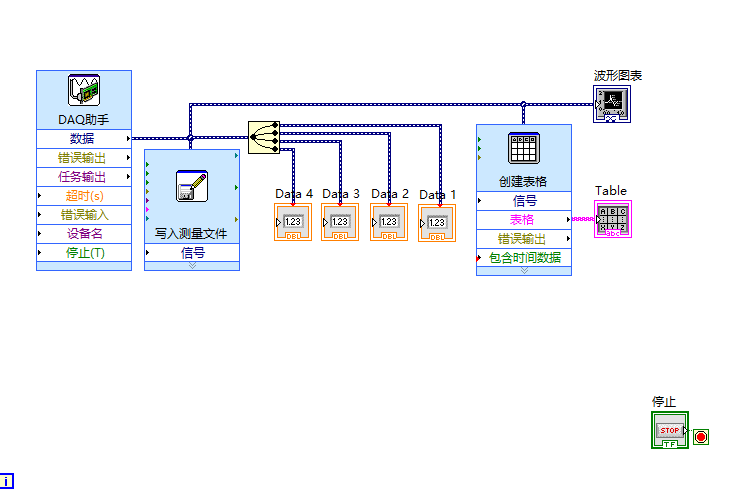
\includegraphics[width=0.45\textwidth]{C8.1/Prog.png}
	}
	\subfloat[操作面板]{\label{fig: pane}
	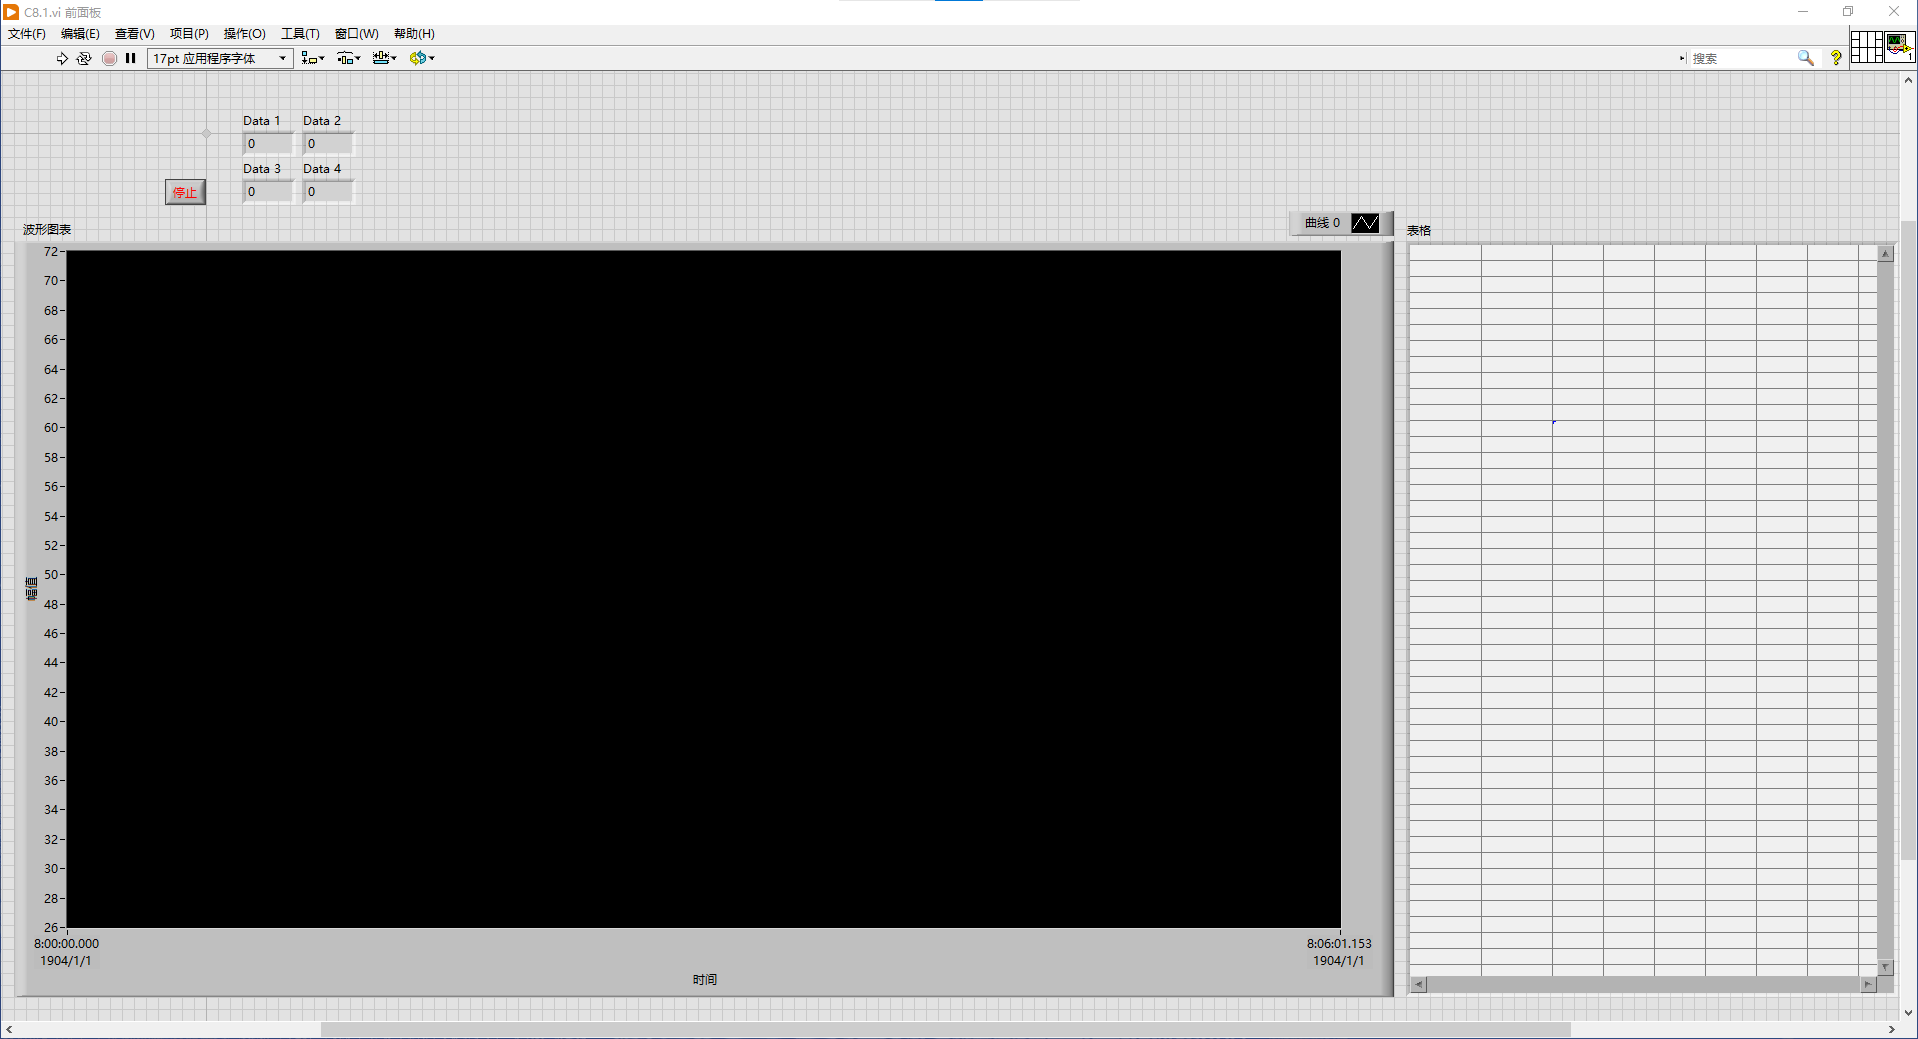
\includegraphics[width=0.45\textwidth]{C8.1/pane.png}
	}
	\caption{}
\end{figure}

测量不同电阻阻值,结果如表\ref{tab: 1}。
\begin{table}[H]
	\centering
	  \begin{tabular}{ccccc}
	  \toprule
	    & $R_1$ & $R_2$ & $R_3$ & $R_4$ \\
		\midrule
	   电阻阻值$\Omega$& 100.00&81.588&42.902&19.846\\
	  \bottomrule
	\end{tabular}
	\caption{电阻阻值测量结果}	  
	\label{tab: 1}
  \end{table}

  用公式$P=I^2 R$分别计算不同阻值电阻在不同电流下的功率,计算结果见表\ref{tab: 2}。
  \begin{table}[H]
	\centering
	  \begin{tabular}{ccccc}
	  \toprule
	  & $R_1$ & $R_2$ & $R_3$ & $R_4$ \\
	  \midrule
	  $P_1$/W&0.04  & 0.032635 & 0.017161 & 0.007938  \\
	  $P_2$/W&0.0625 & 0.050993 & 0.026814 & 0.012404  \\
	  $P_3$/W&0.09  & 0.073429 & 0.038612 & 0.017861  \\
	  $P_4$/W&0.1225 & 0.099945 & 0.052555 & 0.024311  \\
	  $P_5$/W&0.16  & 0.130541 & 0.068643 & 0.031754  \\
	  \bottomrule
	\end{tabular}
	\caption{电阻功率计算结果}	  
	\label{tab: 2}
  \end{table}
  
\subsubsection{同一电流各电阻升温比较}
当电流相同时,不同电阻有不同的升温特性,我们研究了电流为0.02A、0.025A、0.03A、0.035A、和0.04A时不同电阻的升温特性。
结果见图\ref{fig: real_var_I}。
\begin{figure}[H]
	\centering
	\subfloat[I=0.020A]{
	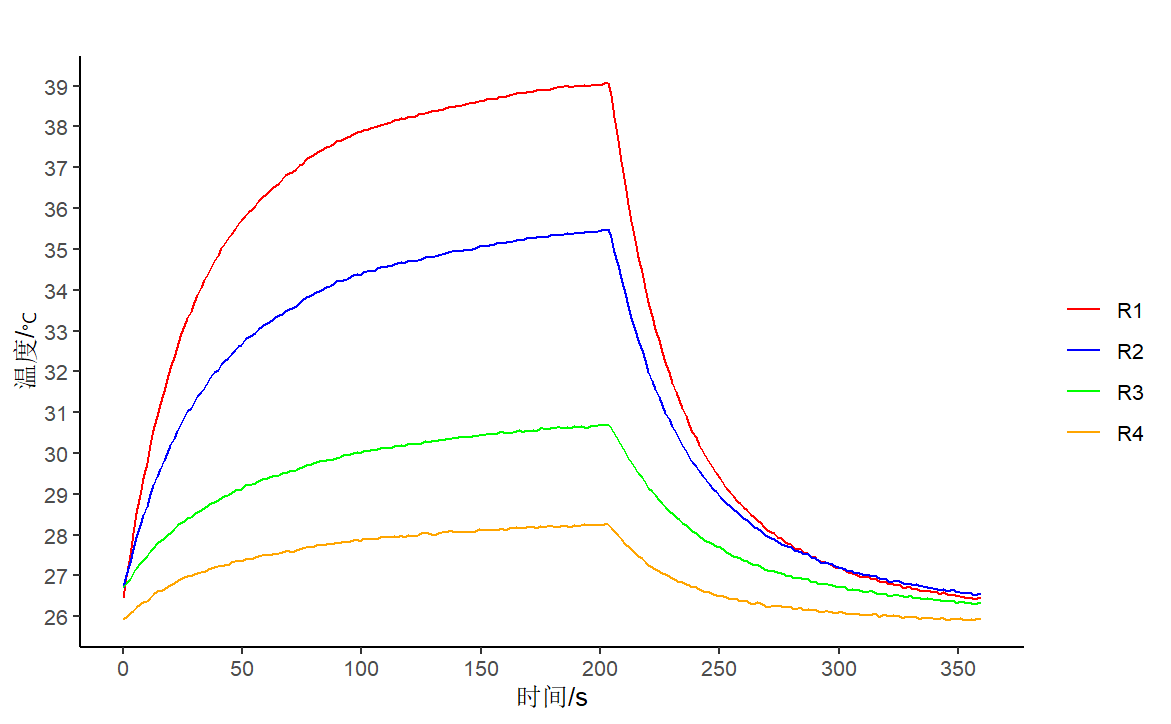
\includegraphics[width=0.3\textwidth]{fig/I_0.02.jpg}
	}%
	\subfloat[I=0.025A]{
	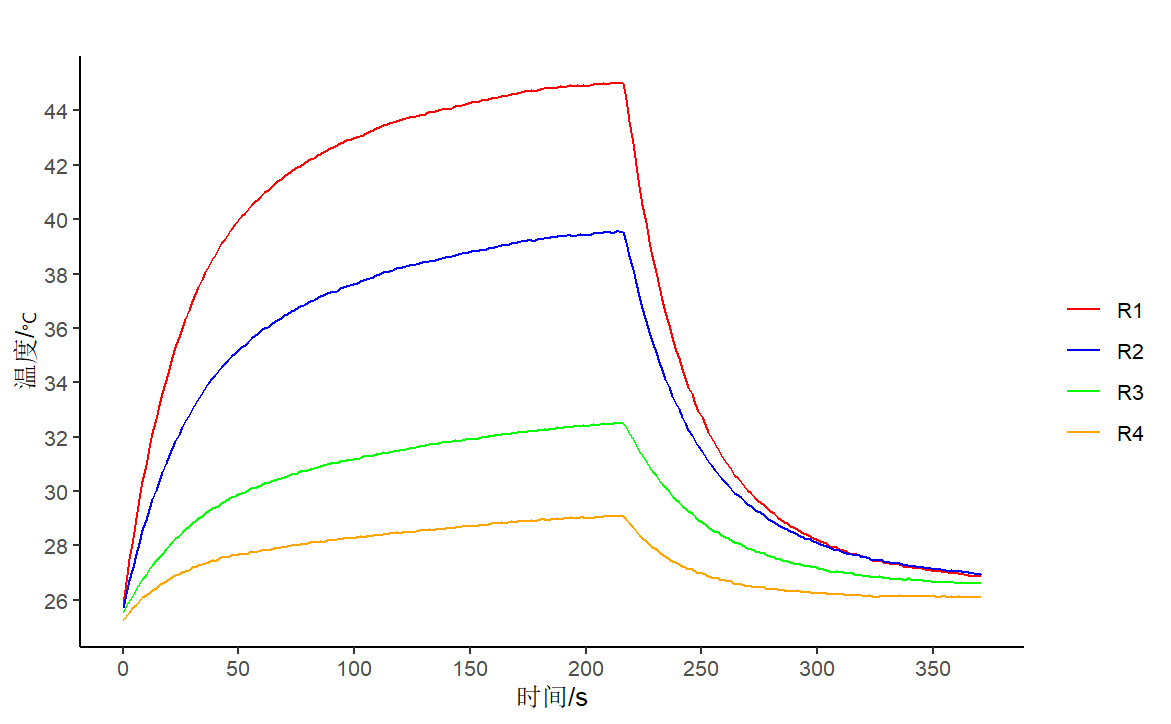
\includegraphics[width=0.3\textwidth]{fig/I_0.025.jpg}
	}%

	\subfloat[I=0.030A]{
	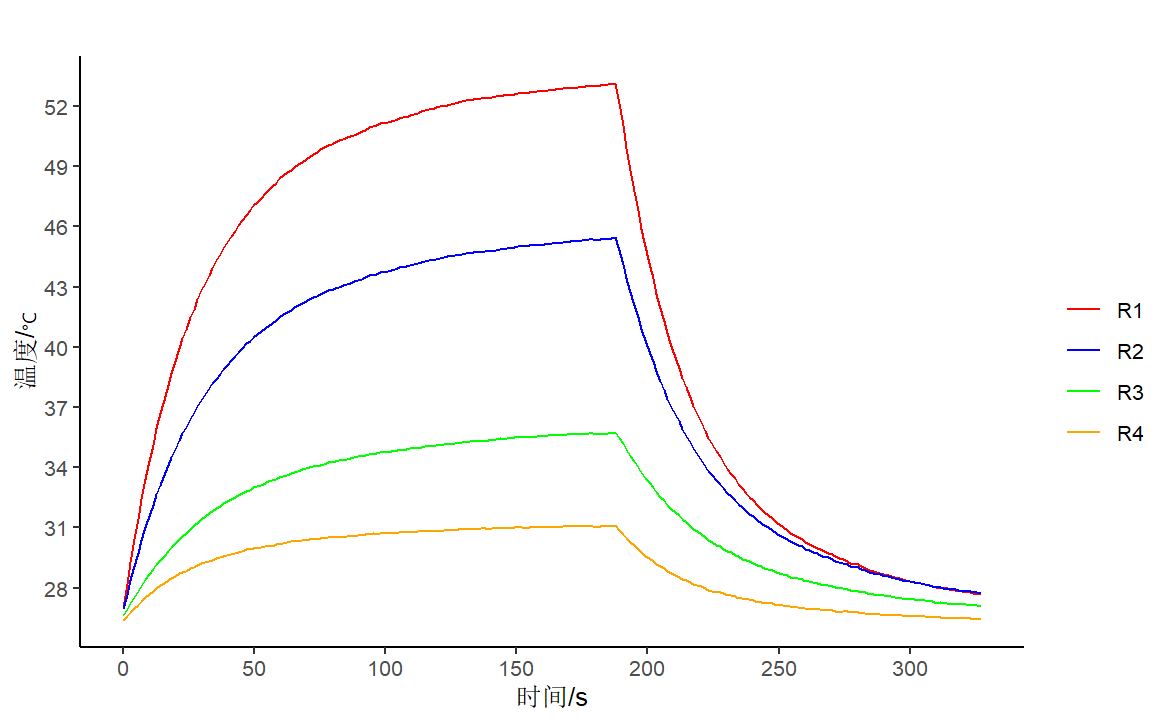
\includegraphics[width=0.3\textwidth]{fig/I_0.03.jpg}
	}%
	\subfloat[I=0.035A]{
	\includegraphics[width=0.3\textwidth]{fig/I_0.035.jpg}
	}%
	\subfloat[I=0.040A]{
	\includegraphics[width=0.3\textwidth]{fig/I_0.04.jpg}
	}%
	\caption{不同电流下各电阻温度随通电时间变化曲线}
	\label{fig: real_var_I}
\end{figure}

\subsubsection{同一电阻各电流升温比较}
当电阻相同时,不同电流下有不同的升温特性。如图\ref{fig:real_var_R}我们研究了电阻为100.00$\Omega$、81.588$\Omega$、42.902$\Omega$和19.846$\Omega$的升温特性。
\begin{figure}[H]
	\centering
	\subfloat[$R_1=100.00\Omega$]{
	\includegraphics[width=0.4\textwidth]{fig/R1.jpg}
	}%
	\subfloat[$R_2=81.588\Omega$]{
	\includegraphics[width=0.4\textwidth]{fig/R2.jpg}
	}%

	\subfloat[$R_3=42.902\Omega$]{
	\includegraphics[width=0.4\textwidth]{fig/R3.jpg}
	}%
	\subfloat[$R_4=19.846\Omega$]{
	\includegraphics[width=0.4\textwidth]{fig/R4.jpg}
	}%
	\caption{不同阻值电阻各功率下温度随通电时间变化曲线}
	\label{fig:real_var_R}
\end{figure}

\begin{table}[H]
	\centering
	  \begin{tabular}{cccccc}
	  \toprule
	  I/A& 0.02 & 0.025 & 0.03 & 0.035 &0.04 \\
	  \midrule
	  $R_1$平衡温度$/^{\circ}C$&39.07593&45.02343&53.16817&62.28702&71.92404\\
	  $R_2$平衡温度$/^{\circ}C$&35.47671&39.55789&45.44987&51.75271&59.07030\\
	  $R_3$平衡温度$/^{\circ}C$&30.69925&32.50692&35.73053&38.55872&42.72767\\
	  $R_4$平衡温度$/^{\circ}C$&28.25695&29.07385&31.09706&32.05471&34.65517\\
	  \bottomrule
	\end{tabular}
	\caption{各电阻平衡温度}	  
	\label{tab: 3}
  \end{table}
  
我们发现,电流相同时,阻值大的电阻升温快,平衡温度高,并且更快达到平衡温度。
对同一电阻而言,电流越大电阻表面温度升高越快,平衡温度更高,同样更快达到平衡温度。
在刚开始加热阶段,电阻表面温度大致与时间成正比,随后曲线趋于平缓,到达平衡温度,到平衡温度所用时间与电阻阻值、
电流大小,初始温度等有关。

\subsection{COMSOL电阻升温模型仿真}

\subsubsection{全铜芯电阻模型}
全铜芯电阻模型即电阻内部材质为铜,图\ref{fig:ac 1}中展示电阻排列,其中左侧显示电阻和电流参数,电阻阻值分别为100.00$\Omega$、81.588$\Omega$、42.902$\Omega$和19.846$\Omega$。
图\ref{fig:ac 2}为运算后电阻内部温度分布。
\begin{figure}[H]
	\centering
	\subfloat[四电阻几何模型]{\label{fig:ac 1}
		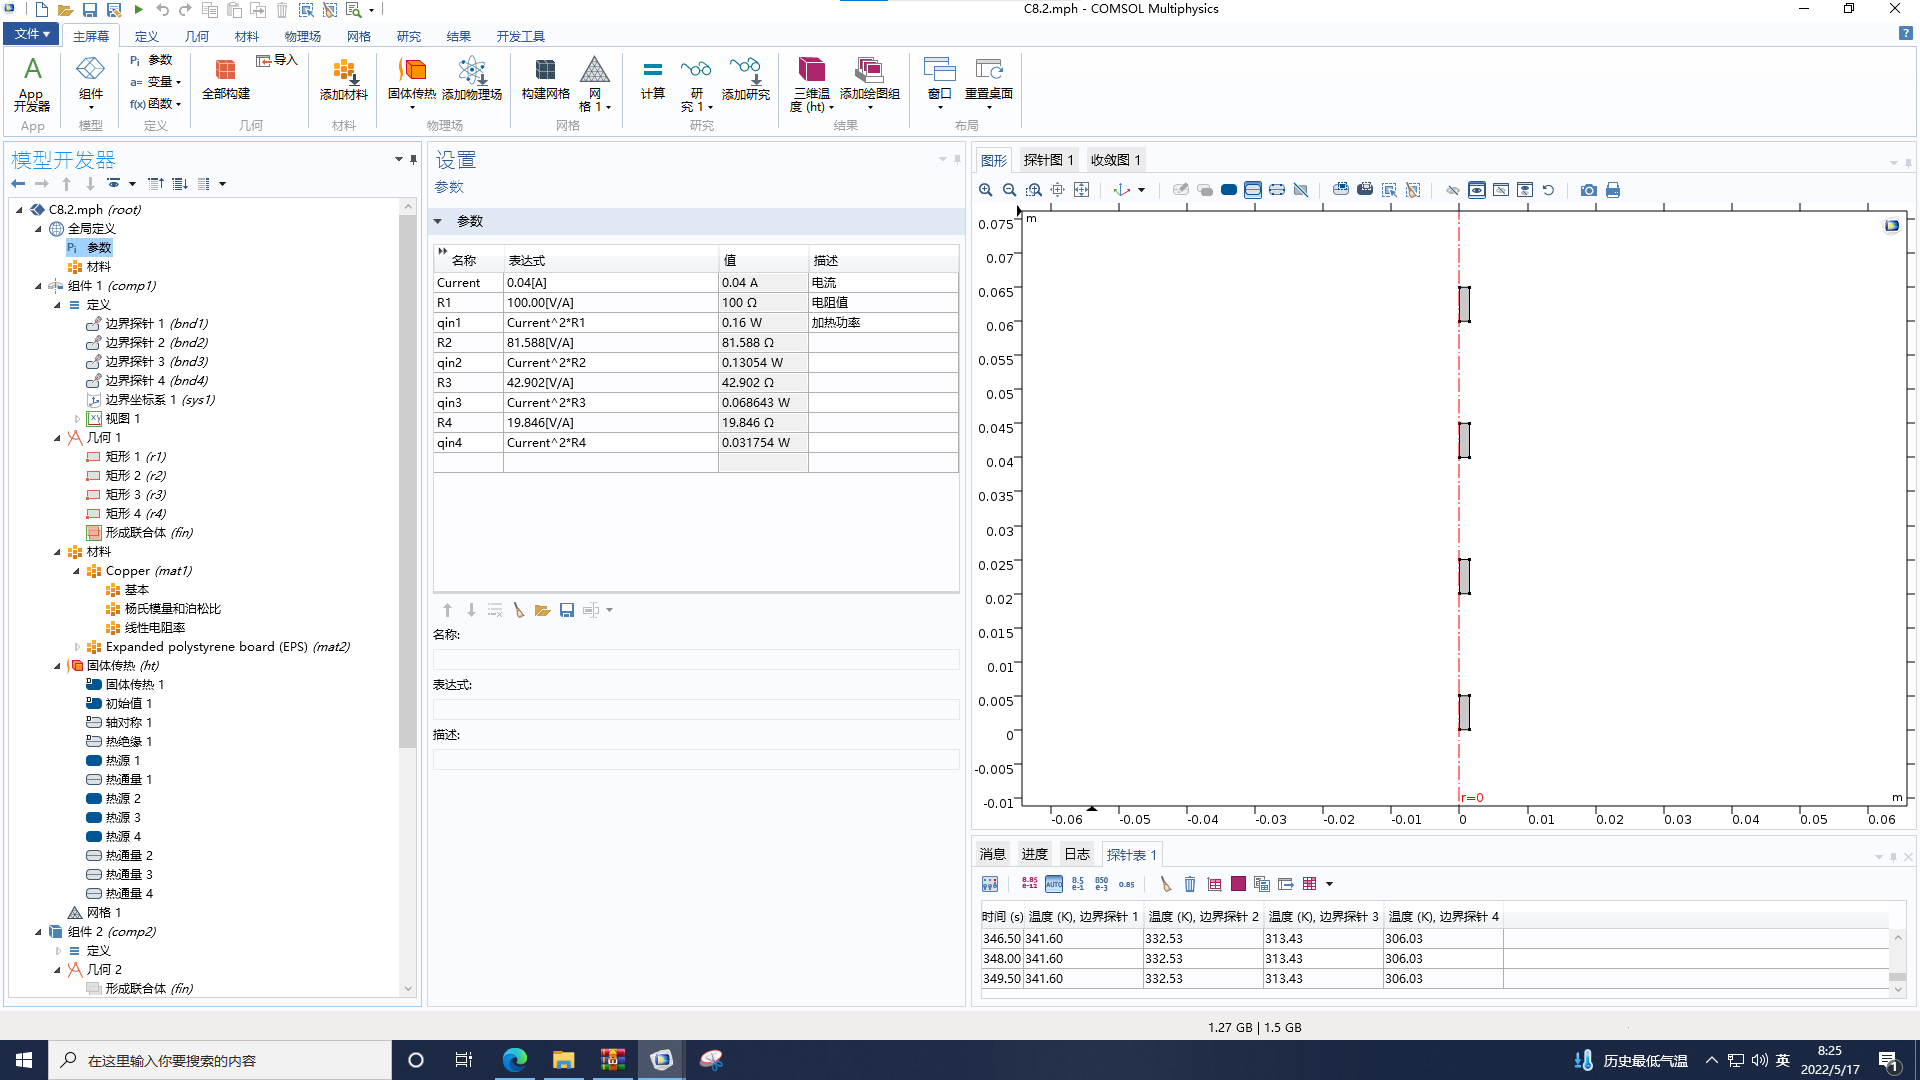
\includegraphics[width=0.5\textwidth]{C8.2/C8.2-v1/para.png}}
	\subfloat[单电阻温度场示例]{\label{fig:ac 2}
		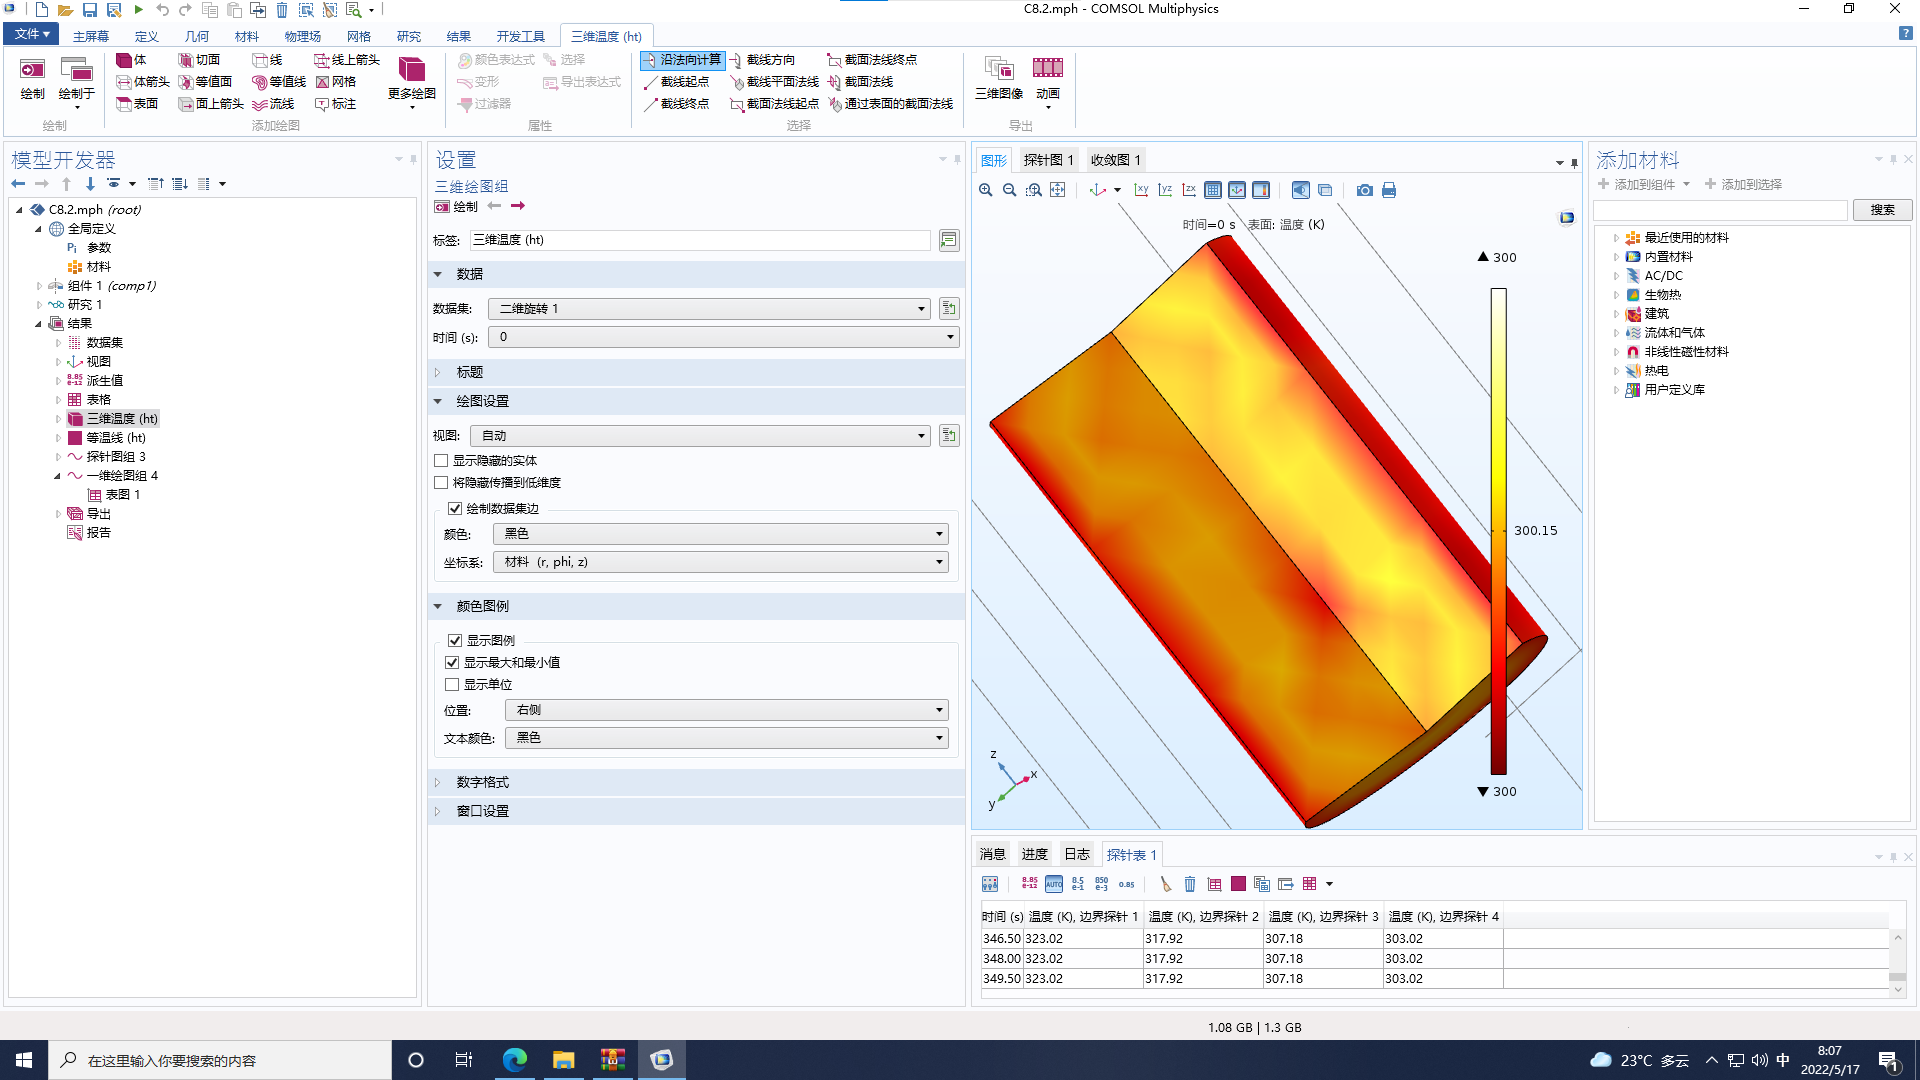
\includegraphics[width=0.5\textwidth]{C8.2/C8.2-v1/0.03/0.030.png}}
	\caption{全铜芯电阻模型工程图}
\end{figure}

取不同电流大小分别运算,得到图\ref{fig: all copper},展示不同电流下各电阻温度随通电时间变化曲线。
\begin{figure}[H]
	\centering
	\subfloat[I=0.020A]{
	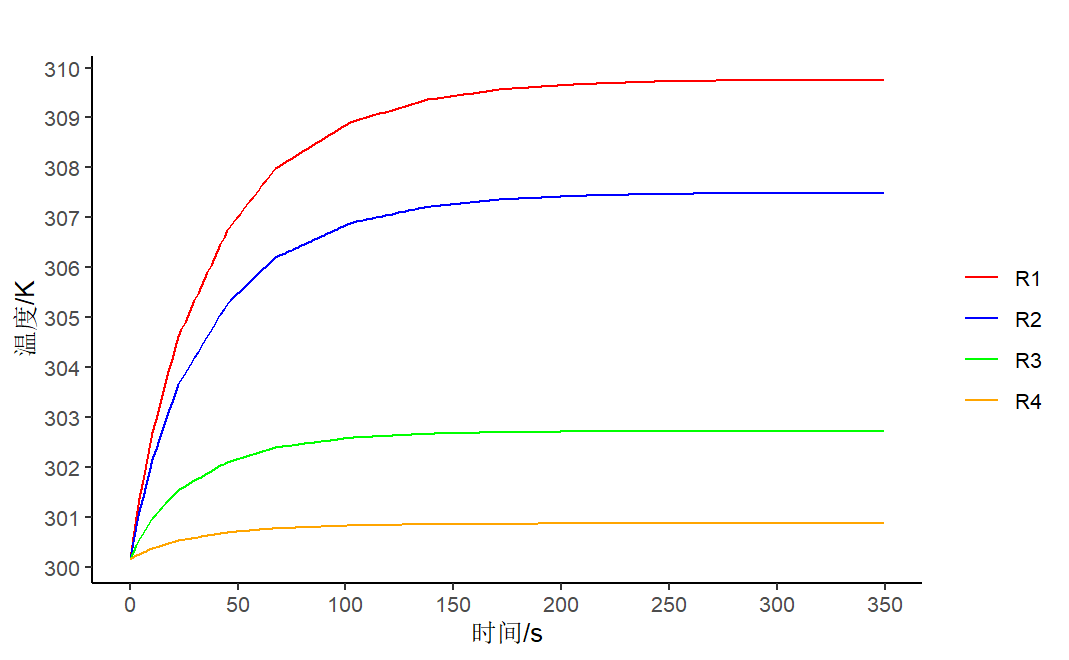
\includegraphics[width=0.3\textwidth]{fig/ac_0.02.png}
	}%
	\subfloat[I=0.025A]{
	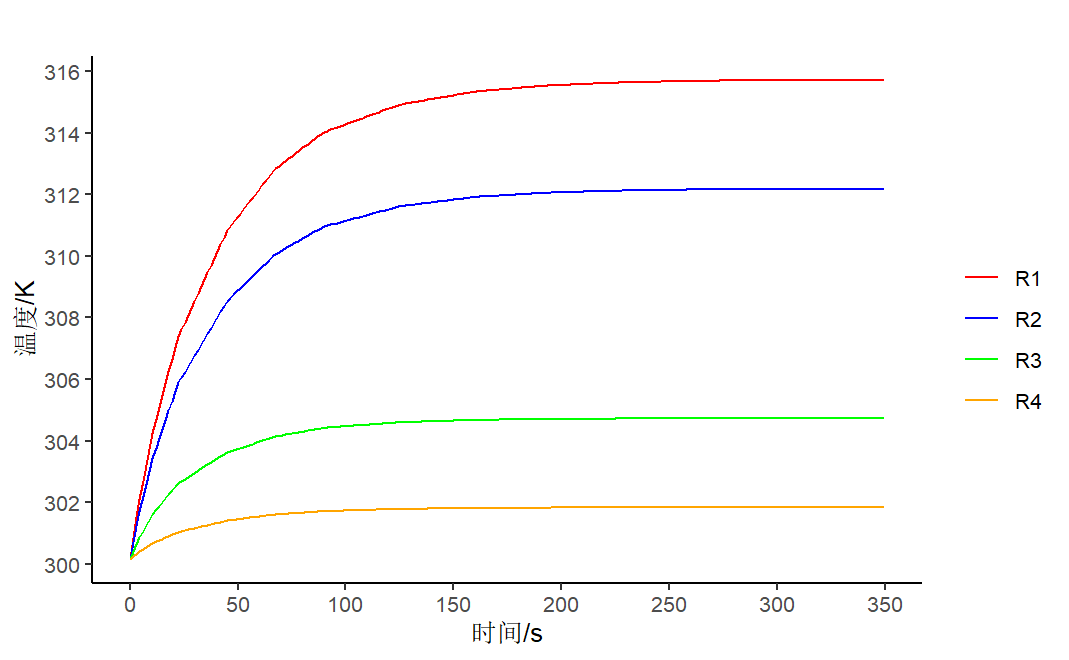
\includegraphics[width=0.3\textwidth]{fig/ac_0.025.png}
	}%

	\subfloat[I=0.030A]{
	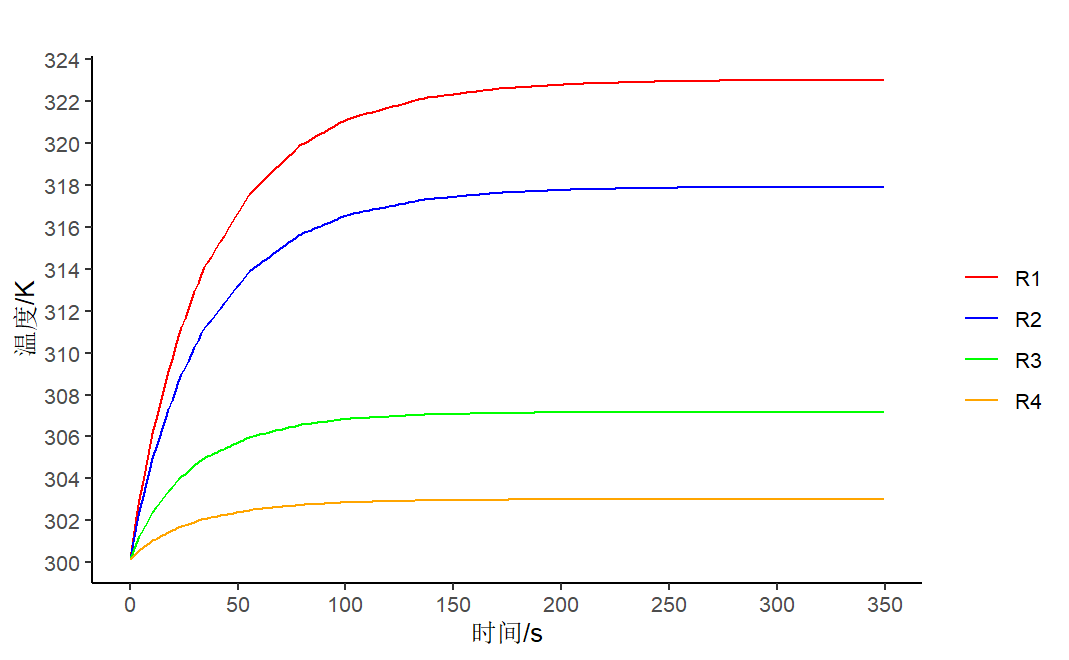
\includegraphics[width=0.3\textwidth]{fig/ac_0.03.png}
	}%
	\subfloat[I=0.035A]{
	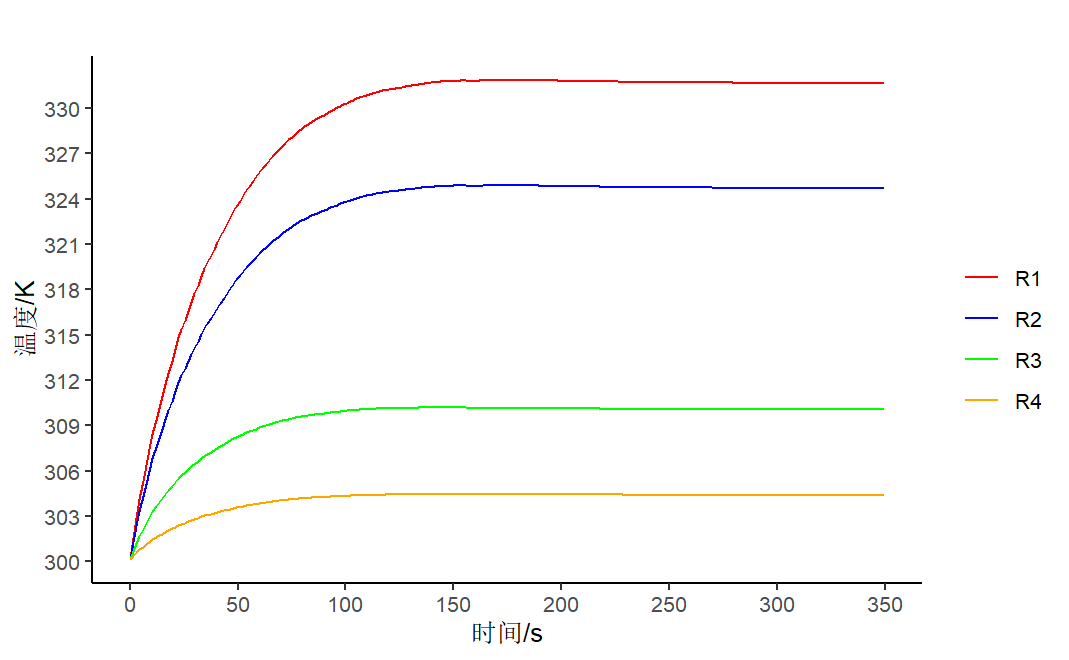
\includegraphics[width=0.3\textwidth]{fig/ac_0.035.png}
	}%
	\subfloat[I=0.040A]{
	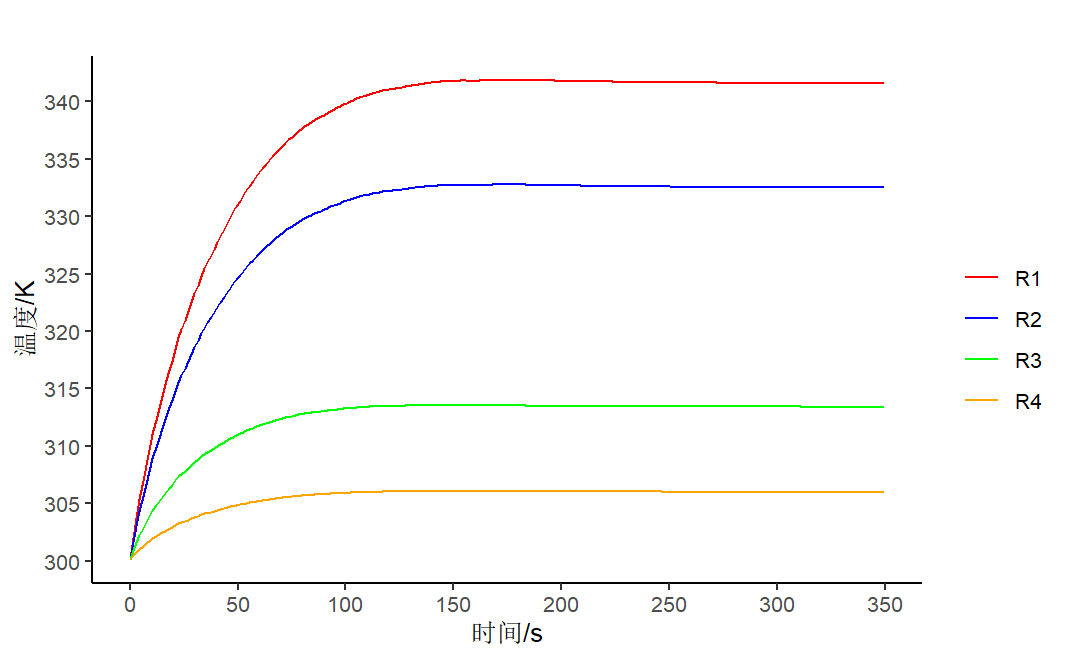
\includegraphics[width=0.3\textwidth]{fig/ac_0.04.png}
	}%
	\caption{不同电流下各电阻温度随通电时间变化曲线}
	\label{fig: all copper}
\end{figure}

不同电流下各电阻温度随通电时间变化曲线形状大致相同,与仿真曲线形状也相类似,但是平衡温度存在差异,仿真结果见表\ref{tab: 4}。
\begin{table}[H]
	\centering
	  \begin{tabular}{cccccc}
	  \toprule
	  I/A& 0.02 & 0.025 & 0.03 & 0.035 &0.04 \\
	  \midrule
	  $R_1$平衡温度$/^{\circ}C$&36.6082 & 42.5746 & 49.8675 & 58.4982 & 68.4466 \\
	  $R_2$平衡温度$/^{\circ}C$&34.3427 & 39.0349 & 44.7703 & 51.5559 & 59.3791 \\
	  $R_3$平衡温度$/^{\circ}C$&29.5702 & 31.5784 & 34.0328 & 36.9343 & 40.2813 \\
	  $R_4$平衡温度$/^{\circ}C$&27.7189 & 28.6858 & 29.8675 & 31.2645 & 32.8761 \\
	  \bottomrule
	\end{tabular}
	\caption{各电阻平衡温度}	  
	\label{tab: 4}
  \end{table}

将实验结果表\ref{tab: 3}与仿真结果表\ref{tab: 4}对比,同一阻值不同电流下的实验和仿真平衡温度结果进行配对t检验,结果如表\ref{tab: 5}。
\begin{table}[H]
	\centering
	  \begin{tabular}{ccccccccc}
		\toprule
		& $R_1$仿真 & $R_1$实验 & $R_2$仿真 & $R_2$实验 & $R_3$仿真 & $R_3$实验 & $R_4$仿真 & $R_4$实验 \\
		\midrule
		平均    & 51.19902 & 54.29572 & 45.81658 & 46.2615 & 34.4794 & 36.04462 & 30.08256 & 31.02755 \\
		方差    & 159.9507 & 173.3768 & 98.90439 & 89.03189 & 18.10102 & 23.0427 & 4.196231 & 6.428171 \\
		观测值   & 5     & 5     & 5     & 5     & 5     & 5     & 5     & 5 \\
		合并方差  & 166.6637 &       & 93.96814 &       & 20.57186 &       & 5.312201 &  \\
		假设平均差 & 0     &       & 0     &       & 0     &       & 0     &  \\
		df    & 8     &       & 8     &       & 8     &       & 8     &  \\
		t Stat & -0.37927 &       & -0.07257 &       & -0.54564 &       & -0.64827 &  \\
		P(T<=t) 单尾 & 0.357178 &       & 0.471965 &       & 0.300096 &       & 0.267484 &  \\
		t 单尾临界 & 1.859548 &       & 1.859548 &       & 1.859548 &       & 1.859548 &  \\
		P(T<=t) 双尾 & 0.714356 &       & 0.94393 &       & 0.600191 &       & 0.534967 &  \\
		t 双尾临界 & 2.306004 &       & 2.306004 &       & 2.306004 &       & 2.306004 &  \\
		\bottomrule	\end{tabular}
	\caption{不同电阻仿真与实验差异检验}	  
	\label{tab: 5}
  \end{table}

  从统计结果可以看出,实验的平衡温度平均值大于仿真结果,其原因可能是仿真时电阻外部未加海绵阻热,散热较快。
  四个电阻仿真与试验配对t检验p值分别为0.714356、0.94393、0.600191、0.534967 ,无明显统计学差异,得出结论仿真实验较符合。

\subsubsection{外层铜片电阻模型}
外层铜片电阻模型即电阻外部由铜片包被,内部为氧化硅晶体,最外层由海绵隔热。几何模型为图\ref{fig:cl 1},加热后温度场为图\ref{fig:cl 2}。
\begin{figure}[H]
	\centering
	\subfloat[四电阻几何模型]{\label{fig:cl 1}
		\includegraphics[width=0.5\textwidth]{C8.2/C8.2-v2/copper.PNG}}
	\subfloat[四电阻温度场示例]{\label{fig:cl 2}
		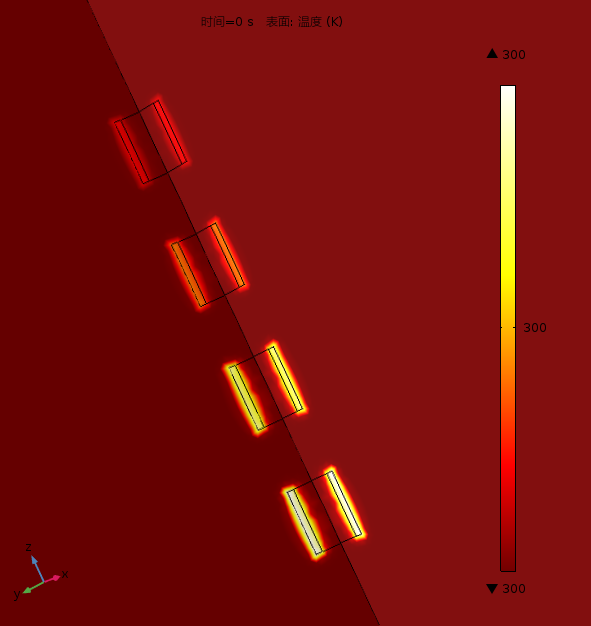
\includegraphics[width=0.25\textwidth]{C8.2/C8.2-v2/0.03/b.png}}
	\caption{外层铜片电阻模型工程图}
\end{figure}

各材料参数如图\ref{fig: mat}:
\begin{figure}[H]
	\centering
	\subfloat[数值参数]{
	\includegraphics[width=0.45\textwidth]{C8.2/C8.2-v2/par.PNG}
	}%
	\subfloat[铜]{
	\includegraphics[width=0.45\textwidth]{C8.2/C8.2-v2/copper.PNG}
	}%

	\subfloat[氧化硅]{
	\includegraphics[width=0.45\textwidth]{C8.2/C8.2-v2/silicon.PNG}
	}%
	\subfloat[海绵]{
	\includegraphics[width=0.45\textwidth]{C8.2/C8.2-v2/spongy.PNG}}
	\caption{材料参数}
	\label{fig: mat}
\end{figure}

不同电流下各电阻温度随通电时间变化曲线如图\ref{fig: copper layer}。
\begin{figure}[H]
	\centering
	\subfloat[I=0.020A]{
	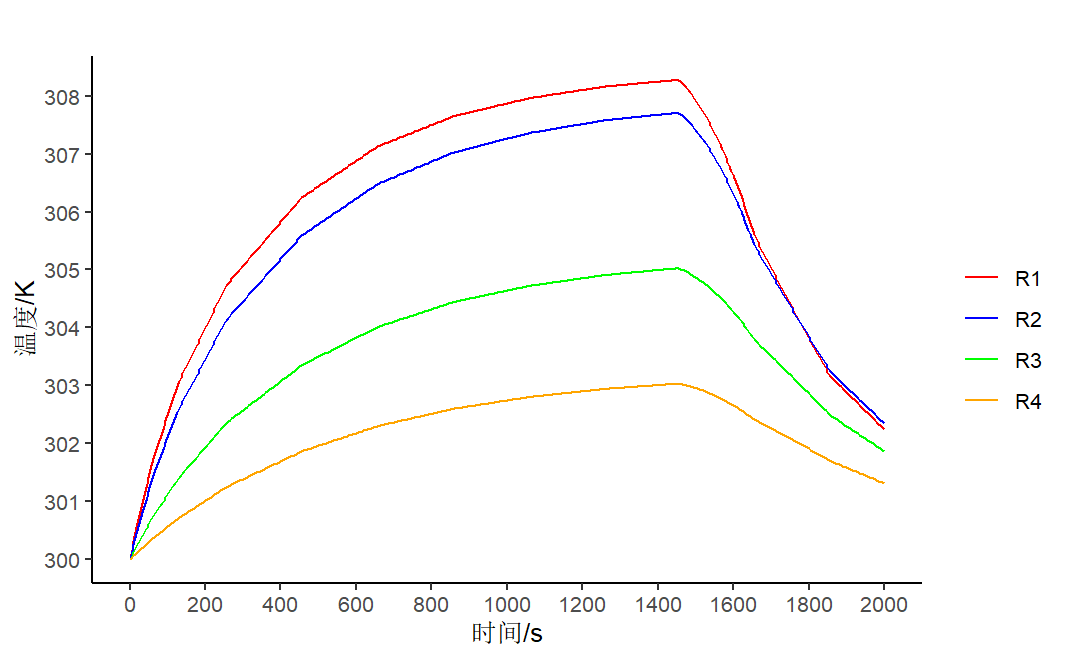
\includegraphics[width=0.3\textwidth]{fig/cl_0.02.png}
	}%
	\subfloat[I=0.025A]{
	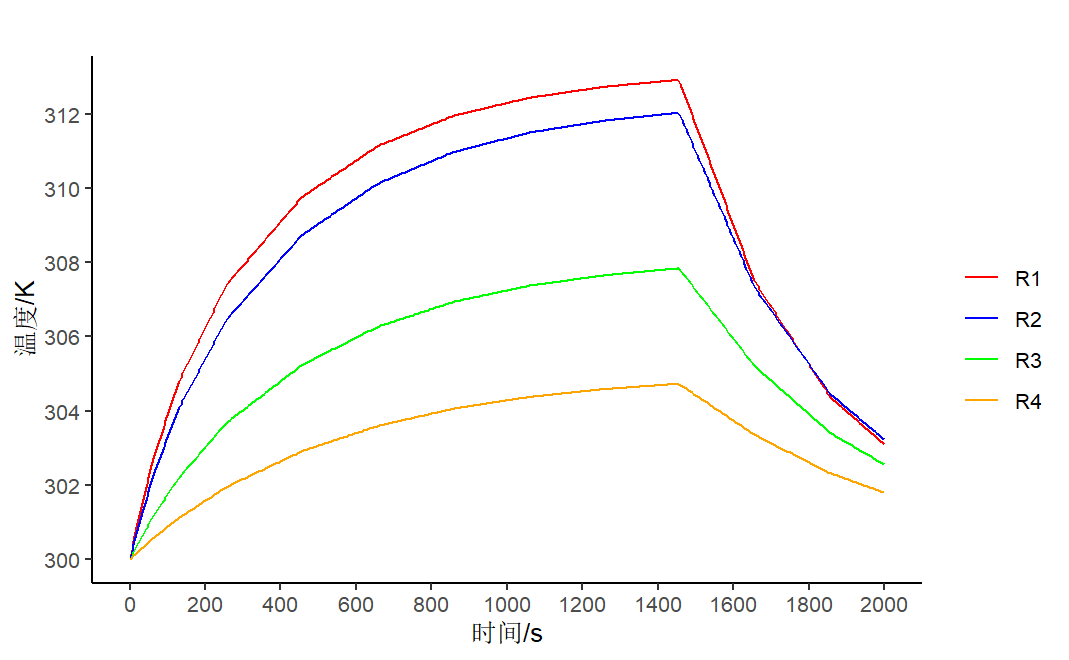
\includegraphics[width=0.3\textwidth]{fig/cl_0.025.png}
	}%

	\subfloat[I=0.030A]{
	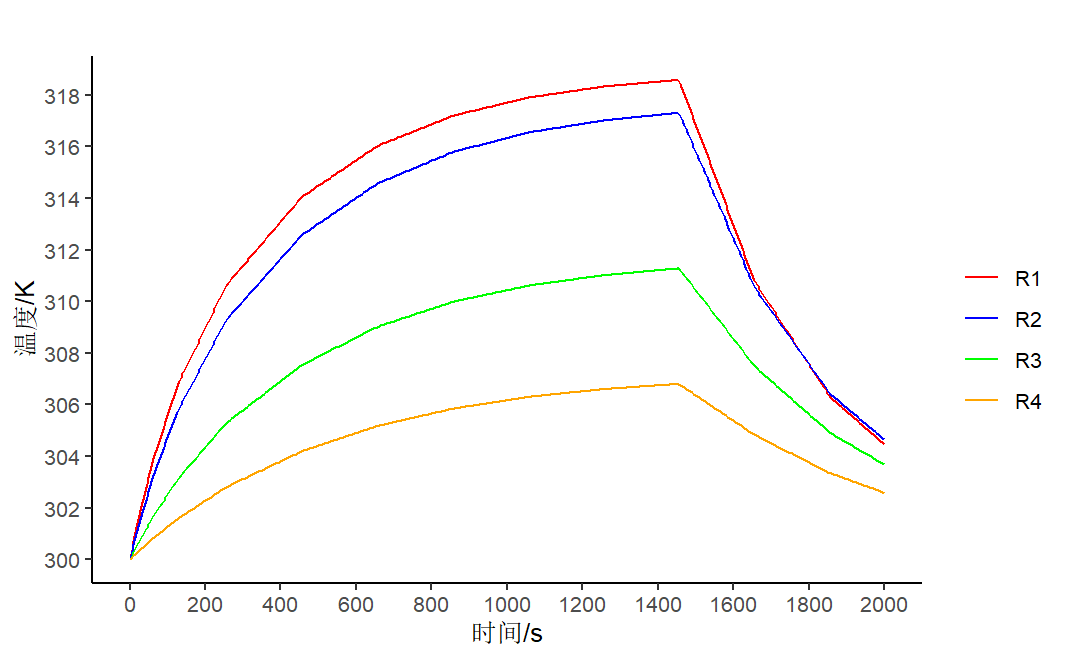
\includegraphics[width=0.3\textwidth]{fig/cl_0.03.png}
	}%
	\subfloat[I=0.035A]{
	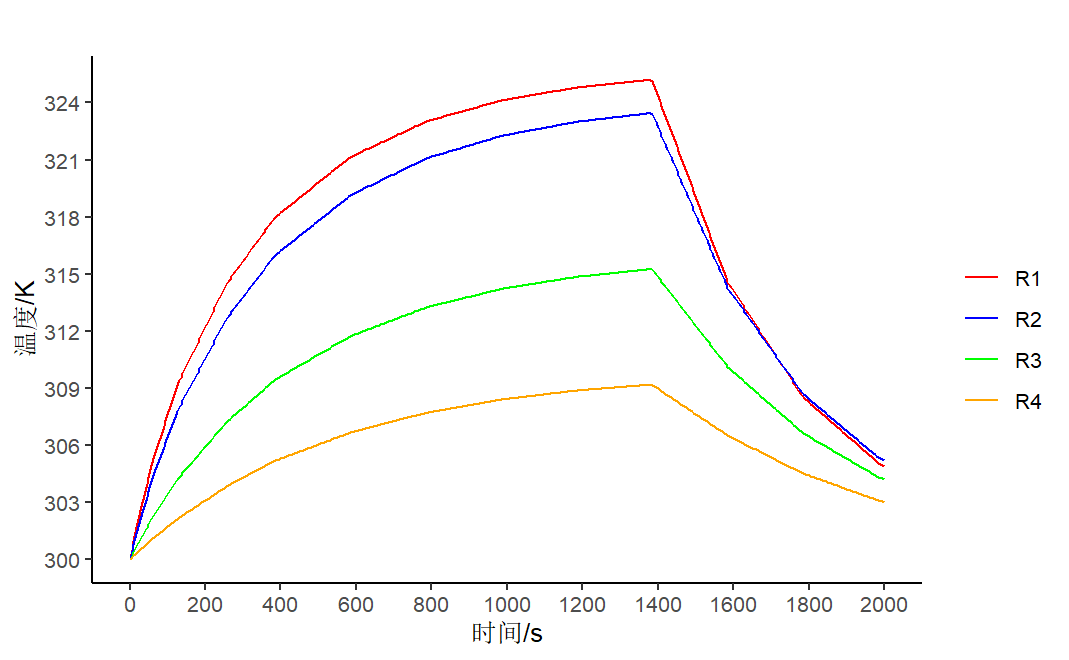
\includegraphics[width=0.3\textwidth]{fig/cl_0.035.png}
	}%
	\subfloat[I=0.040A]{
	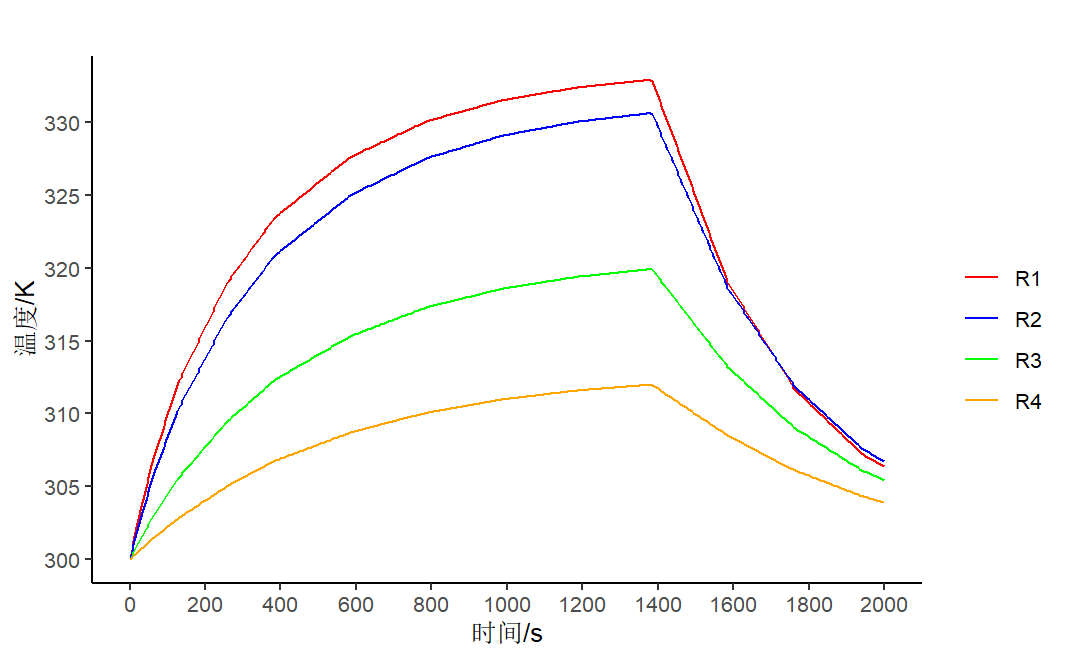
\includegraphics[width=0.3\textwidth]{fig/cl_0.04.png}
	}%
	\caption{不同电流下各电阻温度随通电时间变化曲线}
	\label{fig: copper layer}
\end{figure}

本次实验未看见明显平衡温度,可能由于设置加热时间较短和加热层只有外面的一层铜片,其达到平衡温度所需时间较长所致,故平衡温度整体比全铜电阻模型低。

\subsection{COMSOL热传导模型仿真}
\subsubsection{双样品模拟}
双样品模型由两块材料板组成,外层为加热面。将探针放在外层和中间层测量其温度,修正因子AA为0.85。
\begin{figure}[H]
	\centering
	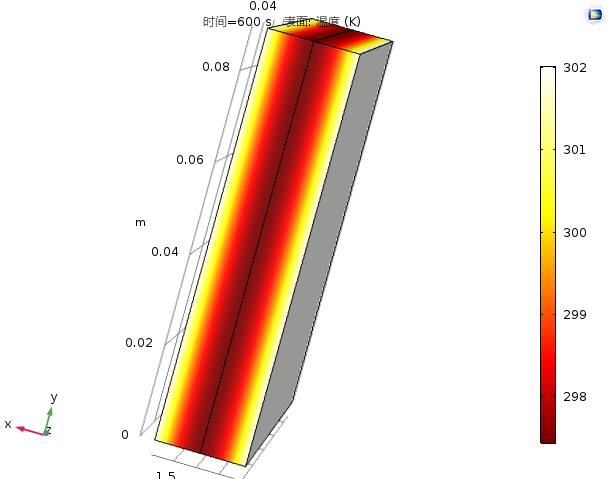
\includegraphics[width=0.4\textwidth]{C8.3/Mod1 glass/b.png}
	\caption{双样品模型及温度分布示例}
	\label{fig: 2}
\end{figure}

有机玻璃和橡胶材料中心面和加热面温度随时间变化曲线如图\ref{fig: Mod1}.
\begin{figure}[H]
	\centering
	\subfloat[玻璃]{
	\includegraphics[width=0.45\textwidth]{fig/m1g.png}
	}%
	\subfloat[橡胶]{
	\includegraphics[width=0.45\textwidth]{fig/m1r.png}
	}%
	\caption{不同材料中心面和加热面温度随时间变化曲线}
	\label{fig: Mod1}
\end{figure}

\subsubsection{四样品模拟}
四样品模型由四块材料板组成,两侧夹层为加热面。将探针放在两侧夹层和中间层测量其温度,修正因子AA为0.85。
\begin{figure}[H]
	\centering
	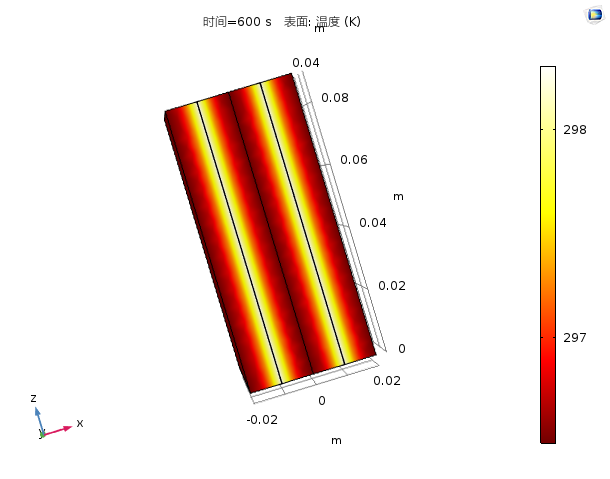
\includegraphics[width=0.4\textwidth]{C8.3/Mod2 rubber/b.png}
	\caption{四样品模型及温度分布示例}
	\label{fig: 4}
\end{figure}

有机玻璃和橡胶材料中心面和加热面温度随时间变化曲线如图\ref{fig: Mod2}.
\begin{figure}[H]
	\centering
	\subfloat[玻璃]{
	\includegraphics[width=0.45\textwidth]{fig/m2g.png}
	}%
	\subfloat[橡胶]{
	\includegraphics[width=0.45\textwidth]{fig/m2r.png}
	}%
	\caption{不同材料中心面和加热面温度随时间变化曲线}
	\label{fig: Mod2}
\end{figure}

\subsubsection{四样品模拟无修正因子模拟(一)}
四样品模型由四块材料板组成,两侧夹层为加热面,并且在样品四周加上阻热层,将探针放在两侧夹层和中间层测量其温度,修正因子AA为1。
\begin{figure}[H]
	\centering
	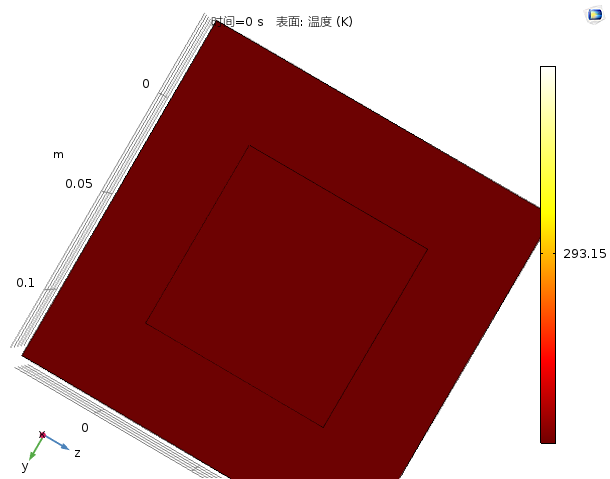
\includegraphics[width=0.4\textwidth]{C8.3/Mod3 glass/b.png}
	\caption{四样品模型及温度分布示例}
	\label{fig: 4_1}
\end{figure}

有机玻璃和橡胶材料中心面和加热面温度随时间变化曲线如图\ref{fig: Mod3}.
\begin{figure}[H]
	\centering
	\subfloat[玻璃]{
	\includegraphics[width=0.45\textwidth]{fig/m3g.png}
	}%
	\subfloat[橡胶]{
	\includegraphics[width=0.45\textwidth]{fig/m4r.png}
	}%
	\caption{不同材料中心面和加热面温度随时间变化曲线}
	\label{fig: Mod3}
\end{figure}

\subsubsection{四样品模拟无修正因子模拟(二)}
四样品模型由四块材料板组成,两侧夹层为加热面,并且在样品四周加上阻热层,前后加上泡沫板,将探针放在两侧夹层和中间层测量其温度,修正因子AA为1。
\begin{figure}[H]
	\centering
	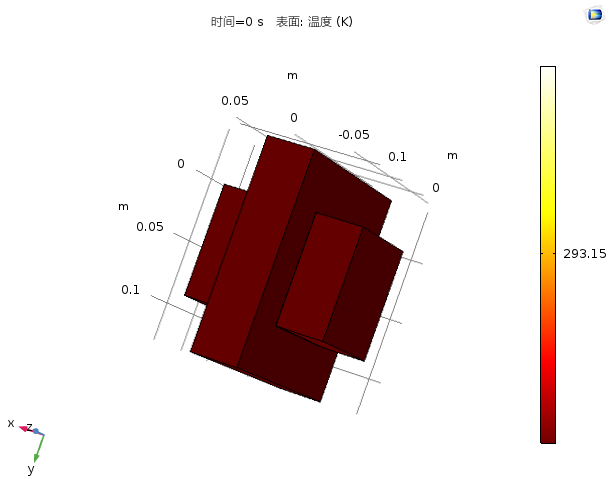
\includegraphics[width=0.4\textwidth]{C8.3/Mod4 glass/b.png}
	\caption{四样品模型及温度分布示例}
	\label{fig: 4_2}
\end{figure}

有机玻璃和橡胶材料中心面和加热面温度随时间变化曲线如图\ref{fig: Mod4}.
\begin{figure}[H]
	\centering
	\subfloat[玻璃]{
	\includegraphics[width=0.45\textwidth]{fig/m3g.png}
	}%
	\subfloat[橡胶]{
	\includegraphics[width=0.45\textwidth]{fig/m4r.png}
	}%
	\caption{不同材料中心面和加热面温度随时间变化曲线}
	\label{fig: Mod4}
\end{figure}

\subsubsection{改变修正因子AA的大小}
\begin{figure}[H]
	\centering
	\subfloat[AA=0.6]{
	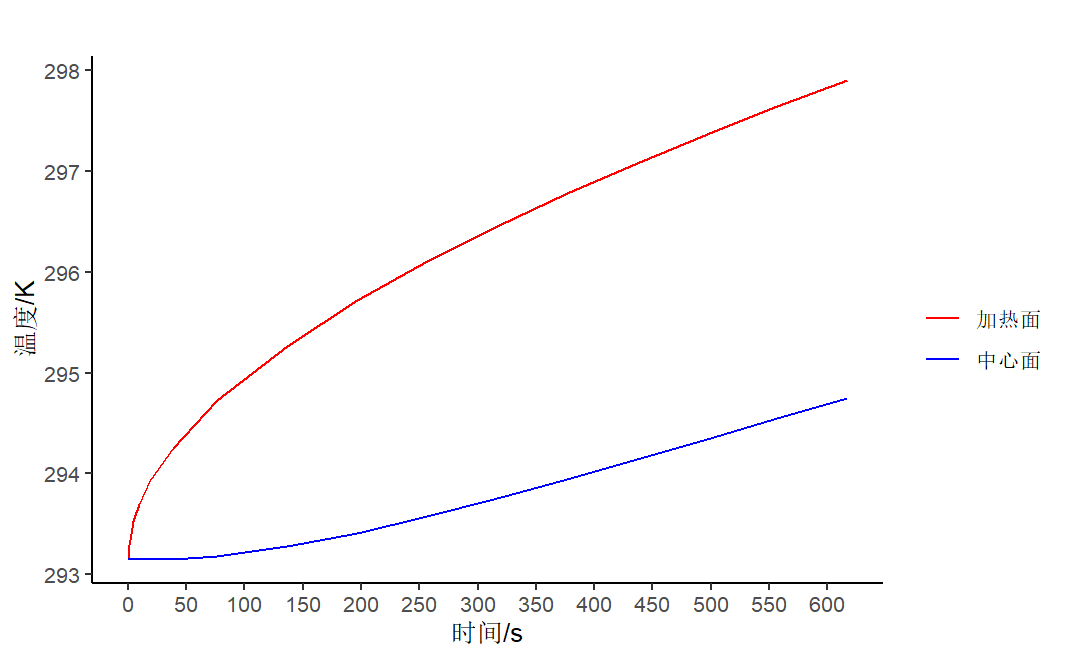
\includegraphics[width=0.33\textwidth]{fig/aa0.6.png}
	}%
	\subfloat[AA=0.85]{
	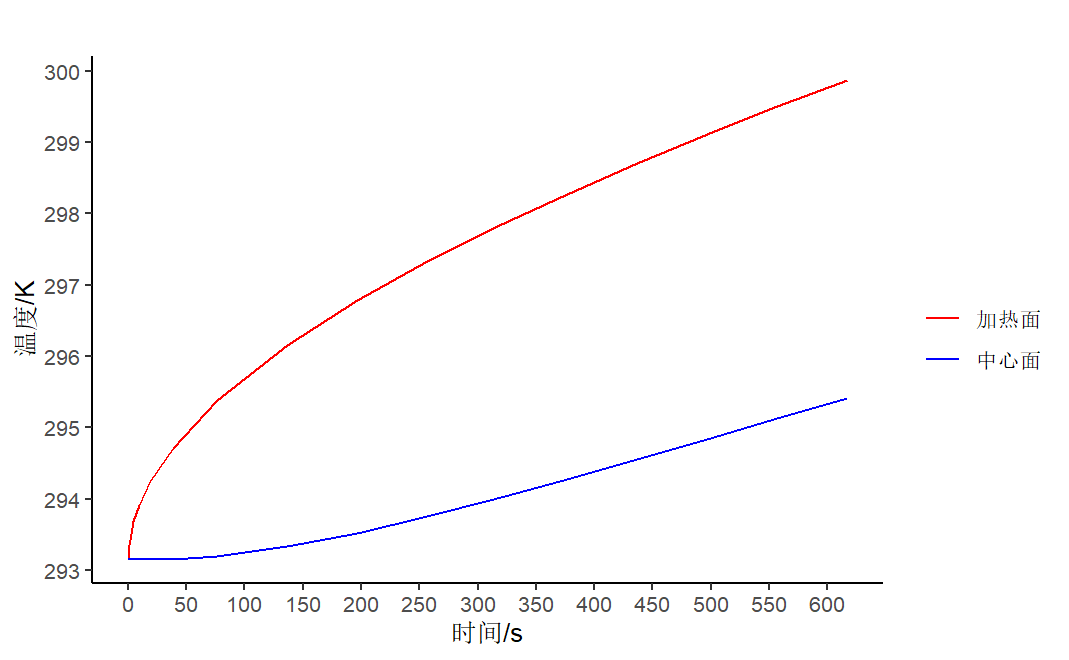
\includegraphics[width=0.33\textwidth]{fig/aa0.85.png}
	}%
	\subfloat[AA=1]{
	\includegraphics[width=0.33\textwidth]{fig/m4g.png}
	}%	
	\caption{改变修正因子AA后玻璃四样品中心面和加热面温度随时间变化曲线}
	\label{fig: Mod5}
\end{figure}

从图\ref{fig: Mod5}中看出,AA越大,升温越快。这与AA代表加热面与样品面积比值的物理意义相符合。

\subsubsection{实验测量四样品中心面和加热面温度随时间变化}
图\ref{fig: Mod6}是实验B2所测得的有机玻璃和橡胶四样品中心面和加热面温度随时间变化图。
\begin{figure}[H]
	\centering
	\subfloat[玻璃]{
	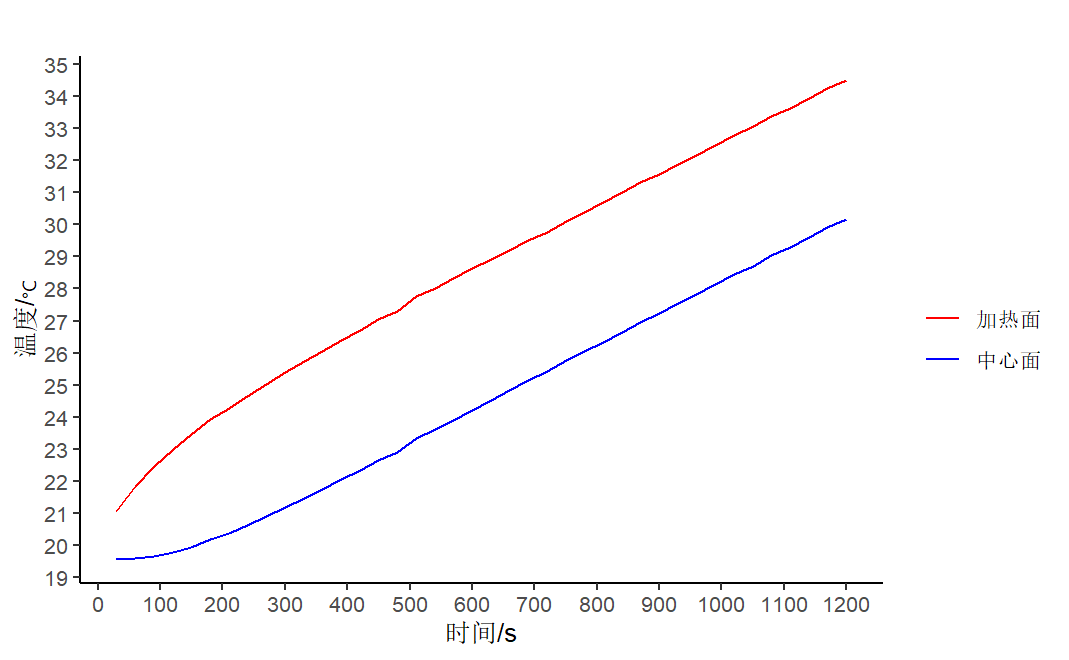
\includegraphics[width=0.45\textwidth]{fig/B2glass.png}
	}
	\subfloat[橡胶]{
	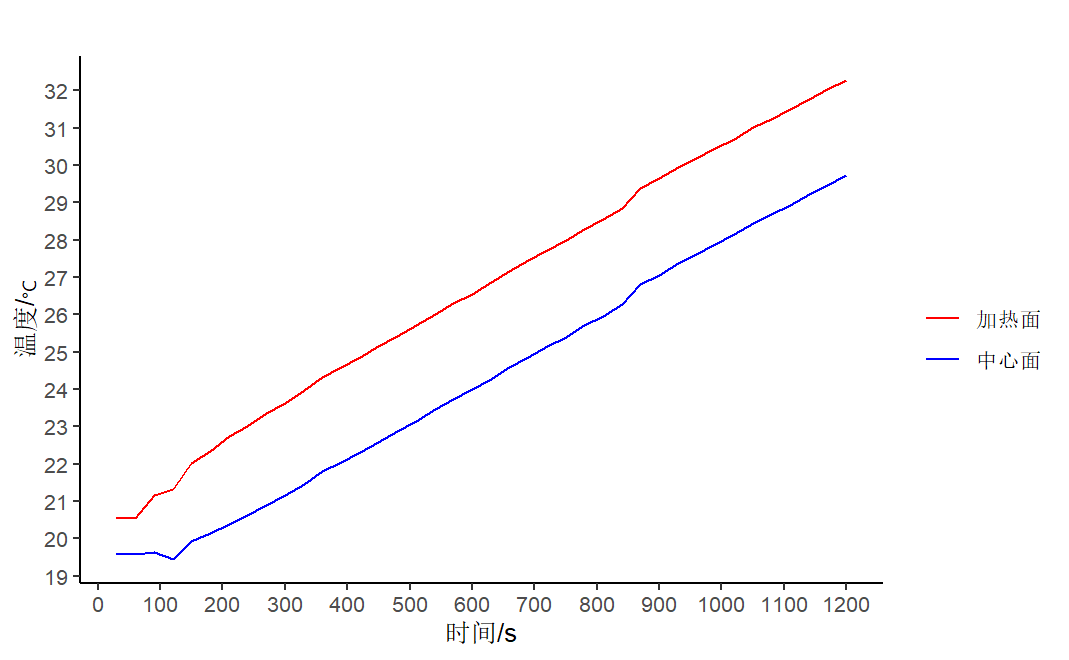
\includegraphics[width=0.45\textwidth]{fig/B2rubber.png}
	}
	\caption{有机玻璃和橡胶四样品中心面和加热面温度随时间变化图}
	\label{fig: Mod6}
\end{figure}

实验中中心面和加热面温度和升温速度普遍高于仿真模拟,并且中心面与加热面温差相对较小。
仅从升温速率上看,最符合实验的仿真是四样品有修正因子仿真。

\section{讨~~~论}
在多通道温度测量实验中平衡温度取断电前一刻温度,即最高温度,对于平衡温度的判断会由对“趋于平缓”的人工判断而产生误差。

COMSOL 电阻升温模型仿真的全铜芯电阻模型与实际电阻材料存在差异,并且外围无海绵隔热,导致与真实实验的误差。
同一阻值不同电流下的实验和仿真平衡温度结果进行配对t检验后得到p值大小不一,由于“p值悖论”我们并不能用p值大小判定仿真与实验结果的相似程度,
故只能以“p>0.05"简陋地判断其无统计学差异。当我们选取外层铜片电阻模型时,或许由于加热铜片过薄,升温较慢,平衡温度较低,始终无法达到
实验的效果。从图上也可以看出“阶跃函数”作用时升温曲线并没有达到平缓的程度,所以此模型有待改进。

COMSOL 热传导模型仿真模型中四样品模型无论有无修正因子有无隔热层,其中心面、加热面温度及其温差均小于实验值,包括升温速率。
其中一个原因是实验材料参数不精确;还有一个可能原因是阻热层与空气热交换极低,近似绝热;当然材料的初温不一致也可能是导致差异的一个原因。

\section{结~~~论}
本实验采用仿真实验和真实实验两种种方式从理论和实践上还原了不同热传导模型。

首先通过多通道温度测量实验发现电流相同时,阻值大的电阻升温快,平衡温度高,并且更快达到平衡温度。对同一电阻而言,电
流越大电阻表面温度升高越快,平衡温度更高,同样更快达到平衡温度。在刚开始加热阶段,电阻表面温度大致
与时间成正比,随后曲线趋于平缓,到达平衡温度,到平衡温度所用时间与电阻阻值、电流大小,初始温度等有关。
  
其次将全铜芯电阻模型的COMSOL仿真与多通道温度测量同一电阻不通电流下的平衡温度做配对t检验。从统计结果可以看出,实验的平衡温度平均值大于仿真结果,其原因可能是仿真时电阻外部未加海绵阻热,
散热较快。四个电阻仿真与试验配对 t 检验 p 值分别为 0.714356、0.94393、0.600191、0.534967 ,无明显统计
学差异,得出结论仿真实验较符合。外层铜片电阻模型未看见明显平衡温度,可能由于设置加热时间较短和加热层只有外面的一层铜片,其达到平衡温
度所需时间较长所致,故平衡温度整体比全铜电阻模型低。

最后在COMSOL上模拟了双样品、四样品含修正因子AA和四样品不含修正因子的两种模型,分别与实验B2所得结果比较,发现实验中中心面和加热面温度和升温速度普遍高于仿真模拟,并且中心面与加热面温差相对较小。仅从升温
速率上看,最符合实验的仿真是四样品有修正因子仿真。
改变修正因子使用有机玻璃进行四样品模拟,发现AA 越大,升温越快。这与 AA 代表加热面与样品面积比值的物理意义相符合。

\newpage
\printbibliography[title=参考文献] 
\clearpage

	 
\section*{\LARGE 附录A}
\section*{【思考题】}
\subsection*{1. 什么是第一类边条件(Dirichlet条件)、第二类边条件(Neumann条件)和第三类变条件(Robin条件),COMSOL能求解哪种边条件的问题?}
答:边值问题中的边界条件的形式多种多样,在端点处大体可以写成这样的形式,Ay+By’=C,若B=0,A$\neq$ 0,则称为第一类边界条件;
B$\neq$0,A=0,称为第二类边界条件;A$\neq$0,B$\neq$0,则称为第三类边界条件。
总体来说,第一类边界条件:给出未知函数在边界上的数值;第二类边界条件:
给出未知函数在边界外法线的方向导数;第三类边界条件:给出未知函数在边界上的函数值与外法向导数的线性组合。
对于COMSOL,只有两种边界条件:第一类边界条件——在端点,待求变量的值被待定。
第二类边界条件——待求变量边界外法线的方向导数被指定。
\subsection*{2. 本实验采用电阻加热模型还有哪些可以改进的地方?}
1.初始值的设置,材料参数越符合真实的物理情况越好。
2.网格设置更细,使得实验结果接近真实值。
3.可考虑添加电阻的外壳材料,如陶瓷壳体、玻璃纤维芯柱、外界填充材
料等,亦可用不同的合金材料代替纯铜材料进行仿真实验。
\subsection*{3. 选择四块板加两个加热膜(共六块板)的情形下,为何膜的通电加热功率要乘以修正因子A?}
加热膜主要材料为聚酰亚胺薄膜,体积约占整个加热膜的六分
之五;通电加热片厚度为0.03mm,体积约占整个加热膜的六分之一,壤嵌在聚酰亚胺薄膜正中间薄
层。当用无加热膜的数学模型时,为了更好模拟真实情况,故膜的通电加热功率要乘以修正因子AA。

\newpage
\section*{\LARGE 附录B}
\section*{【代码示例】}
源代码位于:\url{https://github.com/MoRunbing/Physics_Experiment_Report/tree/main/C8}

其中C8.RData文件包含所需数据集。
\begin{lstlisting}
  ggplot()+
  geom_line(data = mydataset,aes(x = time,y = temperature,colour = "R1"),size=.5)+
  geom_line(data = mydataset,aes(x = time,y = temperature,colour ="R2"),size=.5) + 
  geom_line(data = mydataset,aes(x = time,y = temperature,colour ="R3"),size=.5) + 
  geom_line(data = mydataset,aes(x = time,y = temperature,colour ="R4"),size=.5) + 
  
  scale_colour_manual("",values = c("R1" = "red","R2" = "blue","R3" = "green","R4" = "orange"))+
  scale_y_continuous(breaks=seq(25, 40, 1)) +
  scale_x_continuous(breaks=seq(0, 380, 50))+
  labs(title="plot title", x="x axis", y="y axis")+
  theme_classic()+
  theme(plot.title = element_text(hjust = 0.5))
\end{lstlisting}

\end{document}
